\documentclass[]{article}
\usepackage{lmodern}
\usepackage{amssymb,amsmath}
\usepackage{ifxetex,ifluatex}
\usepackage{fixltx2e} % provides \textsubscript
\ifnum 0\ifxetex 1\fi\ifluatex 1\fi=0 % if pdftex
  \usepackage[T1]{fontenc}
  \usepackage[utf8]{inputenc}
\else % if luatex or xelatex
  \ifxetex
    \usepackage{mathspec}
  \else
    \usepackage{fontspec}
  \fi
  \defaultfontfeatures{Ligatures=TeX,Scale=MatchLowercase}
\fi
% use upquote if available, for straight quotes in verbatim environments
\IfFileExists{upquote.sty}{\usepackage{upquote}}{}
% use microtype if available
\IfFileExists{microtype.sty}{%
\usepackage{microtype}
\UseMicrotypeSet[protrusion]{basicmath} % disable protrusion for tt fonts
}{}
\usepackage[margin=1in]{geometry}
\usepackage{hyperref}
\hypersetup{unicode=true,
            pdftitle={SMDE - Assignment 03},
            pdfauthor={Asaf Badouh, Pau Rodriguez},
            pdfborder={0 0 0},
            breaklinks=true}
\urlstyle{same}  % don't use monospace font for urls
\usepackage{longtable,booktabs}
\usepackage{graphicx,grffile}
\makeatletter
\def\maxwidth{\ifdim\Gin@nat@width>\linewidth\linewidth\else\Gin@nat@width\fi}
\def\maxheight{\ifdim\Gin@nat@height>\textheight\textheight\else\Gin@nat@height\fi}
\makeatother
% Scale images if necessary, so that they will not overflow the page
% margins by default, and it is still possible to overwrite the defaults
% using explicit options in \includegraphics[width, height, ...]{}
\setkeys{Gin}{width=\maxwidth,height=\maxheight,keepaspectratio}
\IfFileExists{parskip.sty}{%
\usepackage{parskip}
}{% else
\setlength{\parindent}{0pt}
\setlength{\parskip}{6pt plus 2pt minus 1pt}
}
\setlength{\emergencystretch}{3em}  % prevent overfull lines
\providecommand{\tightlist}{%
  \setlength{\itemsep}{0pt}\setlength{\parskip}{0pt}}
\setcounter{secnumdepth}{5}
% Redefines (sub)paragraphs to behave more like sections
\ifx\paragraph\undefined\else
\let\oldparagraph\paragraph
\renewcommand{\paragraph}[1]{\oldparagraph{#1}\mbox{}}
\fi
\ifx\subparagraph\undefined\else
\let\oldsubparagraph\subparagraph
\renewcommand{\subparagraph}[1]{\oldsubparagraph{#1}\mbox{}}
\fi

%%% Use protect on footnotes to avoid problems with footnotes in titles
\let\rmarkdownfootnote\footnote%
\def\footnote{\protect\rmarkdownfootnote}

%%% Change title format to be more compact
\usepackage{titling}

% Create subtitle command for use in maketitle
\newcommand{\subtitle}[1]{
  \posttitle{
    \begin{center}\large#1\end{center}
    }
}

\setlength{\droptitle}{-2em}
  \title{SMDE - Assignment 03}
  \pretitle{\vspace{\droptitle}\centering\huge}
  \posttitle{\par}
  \author{Asaf Badouh, Pau Rodriguez}
  \preauthor{\centering\large\emph}
  \postauthor{\par}
  \predate{\centering\large\emph}
  \postdate{\par}
  \date{January 12, 2018}

\begin{document}


\begin{titlepage}

\newcommand{\HRule}{\rule{\linewidth}{0.5mm}}               % horizontal line and its thickness
\newenvironment{bottompar}{\par\vspace*{\fill}}{\clearpage}
\center 
\begin{center}
%----------------------------------------------------------------------------------------
% HEADING SECTIONS
%----------------------------------------------------------------------------------------



\includegraphics{figures/fib-upc-v2-transparent.png}\\[2cm] % Include a department/university logo - this will require the graphicx package
 
%\textsc{\LARGE Polytechnical University of Catalonia}\\[1cm] % Name of your university/college
\textsc{\Large Master in Innovation and Research in Informatics}\\[0.5cm] % Major heading such as course name
\textsc{\large SMDE - Queueing Theory}\\[3cm] % Minor heading such as course title

%----------------------------------------------------------------------------------------
% TITLE SECTION
%----------------------------------------------------------------------------------------

\HRule \\[0.4cm]
{ \huge \bfseries Evaluation of G/G/1 Systems}\\[0.4cm] % Title of your document
\HRule \\[1.5cm]
 
%----------------------------------------------------------------------------------------
% AUTHOR SECTION
%----------------------------------------------------------------------------------------
\begin{bottompar}
\begin{minipage}{0.5\textwidth}
\begin{flushleft} \large
\emph{Authors:}\\
Asaf Badouh \\ Pau Rodríguez Esmerats % Your name
\end{flushleft}
\end{minipage}
~
\begin{minipage}{0.4\textwidth}
\begin{flushright} \large
\emph{Professor:} \\
Esteve Codina
\end{flushright}
\end{minipage}\\[2cm]

%----------------------------------------------------------------------------------------
% DATE SECTION
%----------------------------------------------------------------------------------------

{\large \today}\\[2cm] % Date, change the \today to a set date if you want to be precise
\end{bottompar}
\end{center}
\end{titlepage}

\tableofcontents
\pagebreak


\subsection{Initial analysis}\label{initial-analysis}

We execute a small simulation with 10.000 clients to verify that the
simulation is running correctly. Our probability distribution for
modelling the services times is a Lognormal with \(\sigma=1.4286\). To
obtain the other parameter of the distribution, the \(\mu\), we choose
the first traffic factor, \(\rho=0.4\), which allows us to compute the
\(\mu\).\\
\[  \rho = { \lambda \over {s\mu}} = { E[x] \over E[\tau] } = e^{\mu} \cdot { e^{\sigma^{2} \over 2} \over E[x] } \Rightarrow \mu = ln \left( { \rho \over e^{ \sigma^{2} \over 2 } } \cdot E[\tau]  \right) \]
The resulting \(\mu\) is 2.4070657.

In our simulation, the arrival times are defined by a Normal
distributioni with parameters \(\mu=77, \sigma=15\). We generate 10.000
clients int the simulation, and analyse the service times.

The histogram of the service times is shown below:

\begin{center}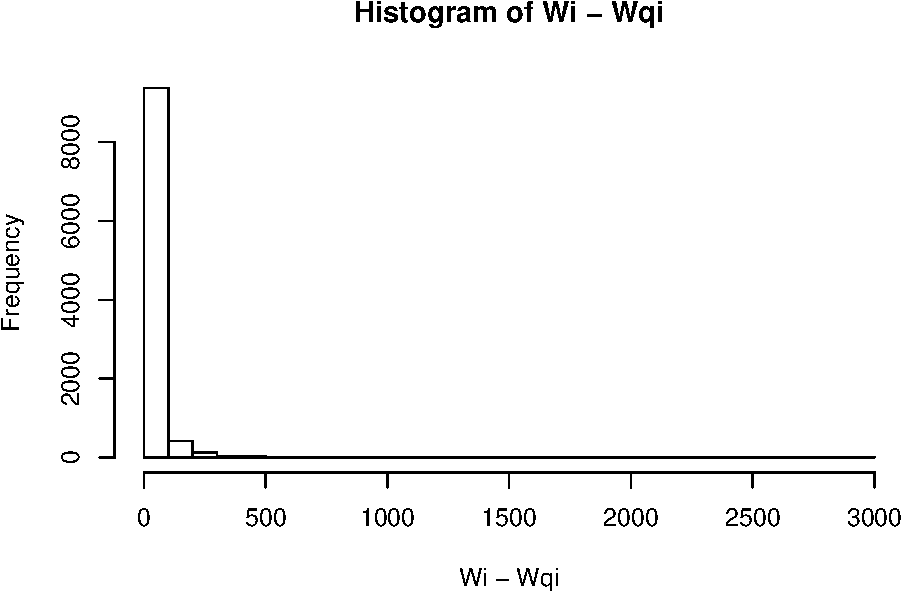
\includegraphics[width=0.5\linewidth]{003_files/figure-latex/unnamed-chunk-7-1} \end{center}

The mean and sample variance of the services times are the following:

\begin{enumerate}
\def\labelenumi{\arabic{enumi}.}
\tightlist
\item
  Mean of the service times: \(W_{s_{avg}}\)=29.9956819
\item
  Standard deviation of the service times: \(W_{s_{std}}\)=70.4786576
\item
  Coeficient of variation: \(C_{x}={ \sigma_{x} \over E[x] }\)=2.3496268
\end{enumerate}

The Theoretical values for a Lognormal with \(\mu\)=2.4070657 and
\(\sigma\)=1.4286 are the follwing:

\begin{enumerate}
\def\labelenumi{\arabic{enumi}.}
\tightlist
\item
  Mean of the service times: \(E[x]\)=30.8
\item
  Standard deviation of the service times: \(sqrt{Var[x]}\)=79.7090561
\item
  Coeficient of variation: \(C_{x}={ \sigma_{x} \over E[x] }\)=2.5879564
\end{enumerate}

We observe that the sample statistics are close to the theoretical
values. Our simulation can be considered to be correct.

\subsection{\texorpdfstring{Allen Cuneen's aproximation formula for
\(W_{q}\) and
\(L_{q}\)}{Allen Cuneen's aproximation formula for W\_\{q\} and L\_\{q\}}}\label{allen-cuneens-aproximation-formula-for-w_q-and-l_q}

For each loading factor \(\rho\), we derive the required \(\mu\) value
for the Lognormal distribution: \[  s = 1 \]
\[  \lambda = { 1 \over E[\tau] } \] \[  \mu = {1 \over E[x]} \]
\[  E[x] = m \cdot e^{\sigma^{2} \over 2} = e^{\mu + {\sigma^{2} \over 2} }\]
\[  \rho = { \lambda \over {s\mu}} = { E[x] \over E[\tau] } = e^{\mu} \cdot { e^{\sigma^{2} \over 2} \over E[x] } \Rightarrow \mu = ln \left( { \rho \over e^{ \sigma^{2} \over 2 } } \cdot E[\tau]  \right) \]

We use the Allen Cuneen's approximation formula for \(L_{q}\): \[
  L_{q} \approx L_{q_{M/M/1}} \cdot \left( C_{\tau}^{2} + C_{x}^{2} \over 2  \right) \\
\] With: \[
C_{x} = \sqrt{ \omega - 1} =  \sqrt{ e^{\sigma^{2}} - 1} \\
C_{\tau} = { \sigma_{\tau} \over E[\tau] }
\] And derive \(W_{q}\): \[
  W_{q} = { L_{q} \over \lambda }
\]

Using the Allen Cuneen's approximation formula, we can compute the
\(W_{q}\) and \(L_{q}\) for each loading factor:

\begin{longtable}[]{@{}llll@{}}
\toprule
\(\rho\) & \(\mu\) & \(W_{q}\) & \(L_{q}\)\tabularnewline
\midrule
\endhead
0.4 & 2.4070657 & 69.1507968 & 0.8980623\tabularnewline
0.7 & 2.9666815 & 423.5486306 & 5.5006316\tabularnewline
0.85 & 3.1608375 & 1249.0362678 & 16.2212502\tabularnewline
0.925 & 3.2453949 & 2958.3575269 & 38.4202276\tabularnewline
\bottomrule
\end{longtable}

\subsection{Simulation}\label{simulation}

First, for each \(\rho\), we're going to calculate what is the amount of
clients needed to get in the steady state of the waiting system.

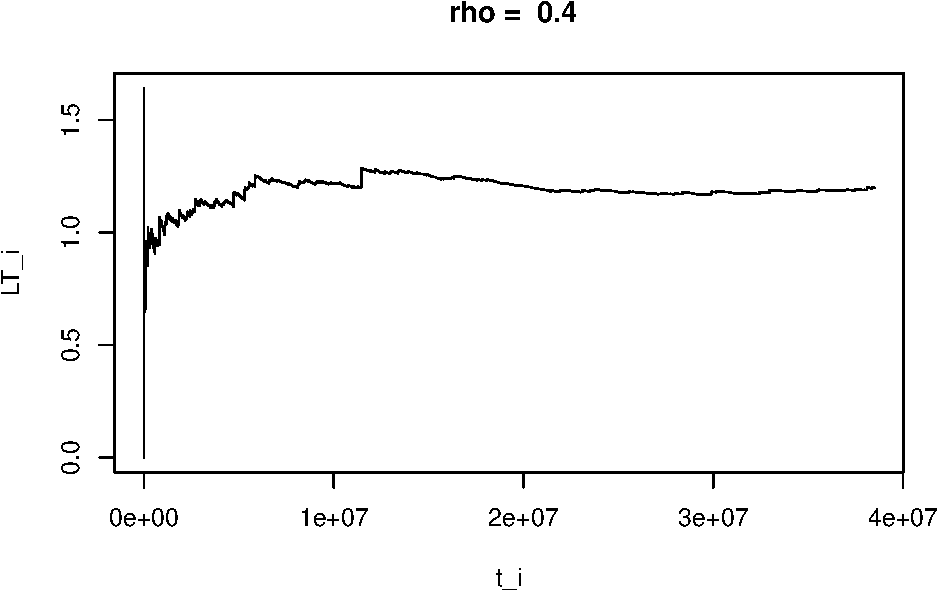
\includegraphics{003_files/figure-latex/unnamed-chunk-11-1.pdf}
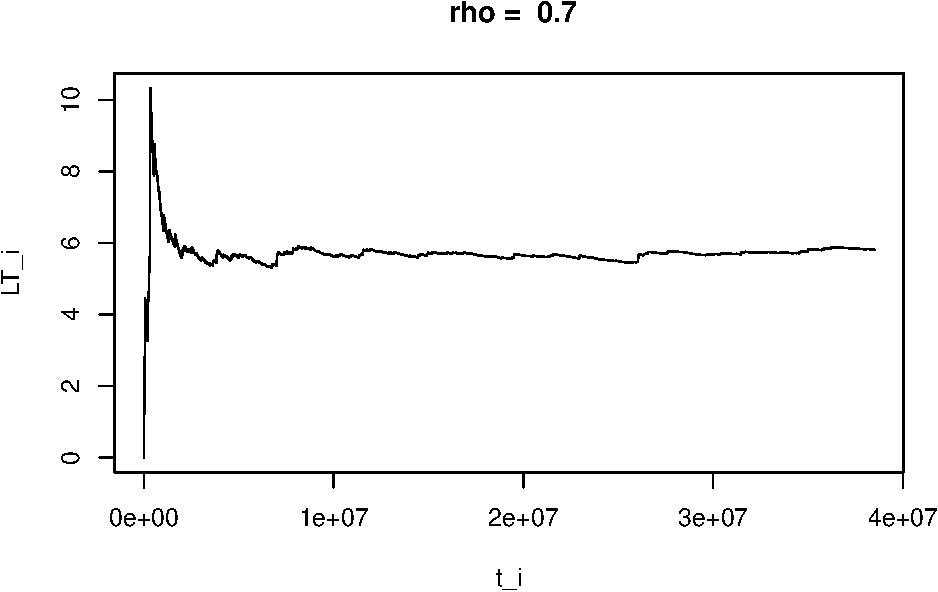
\includegraphics{003_files/figure-latex/unnamed-chunk-11-2.pdf}
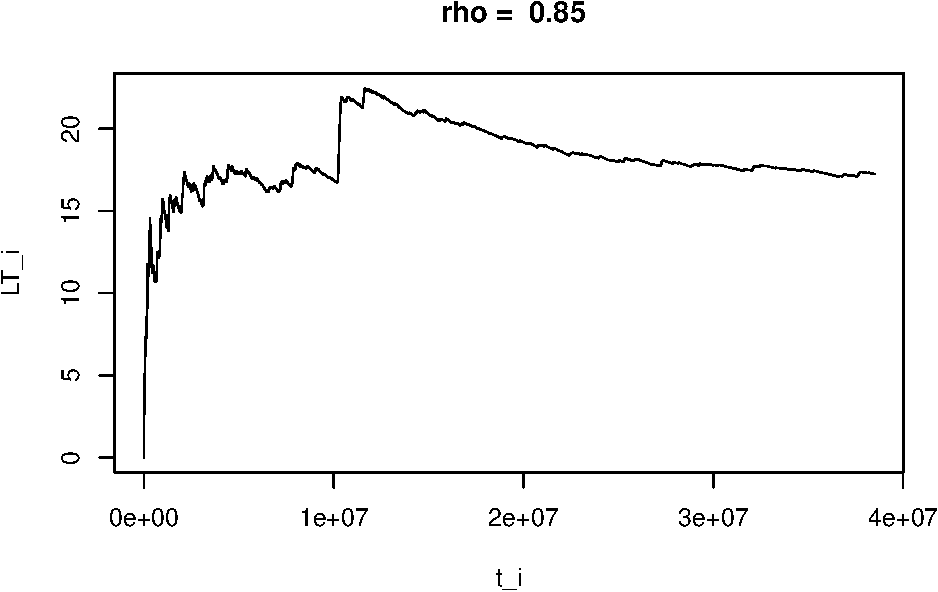
\includegraphics{003_files/figure-latex/unnamed-chunk-11-3.pdf}
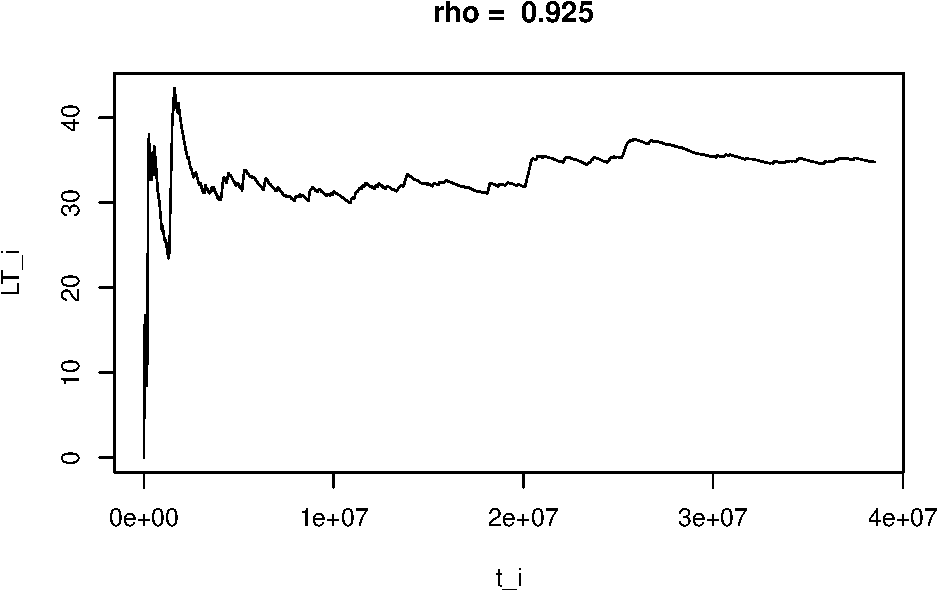
\includegraphics{003_files/figure-latex/unnamed-chunk-11-4.pdf}

We observe that, apart from the simulation with loading factor 0.4, the
other simulations have not attained the steady state.

If we repeat the simulations with a number of clients between 200000 and
500000, the steady state is attained with all loading factors. We have
not tested more than 500000 clients.

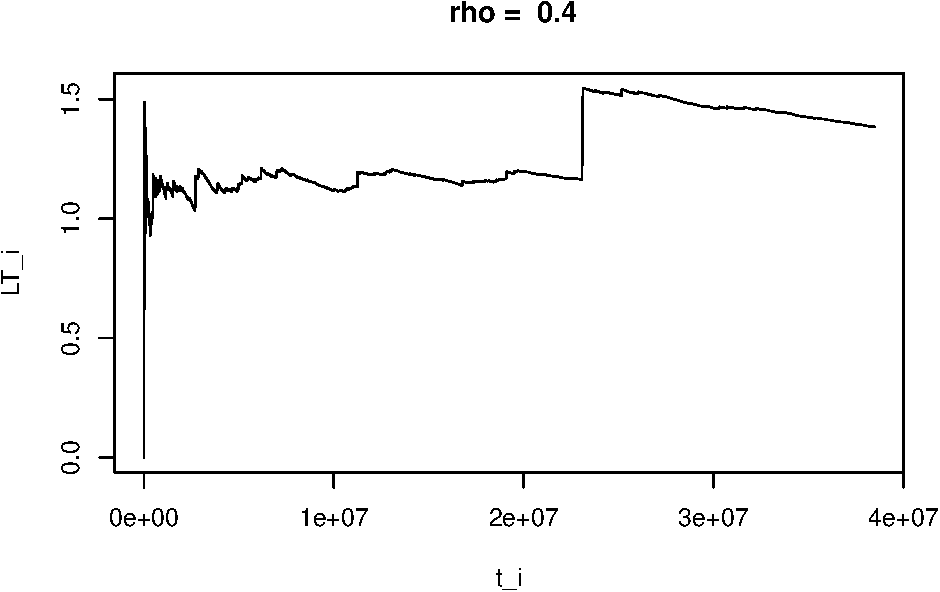
\includegraphics{003_files/figure-latex/unnamed-chunk-12-1.pdf}
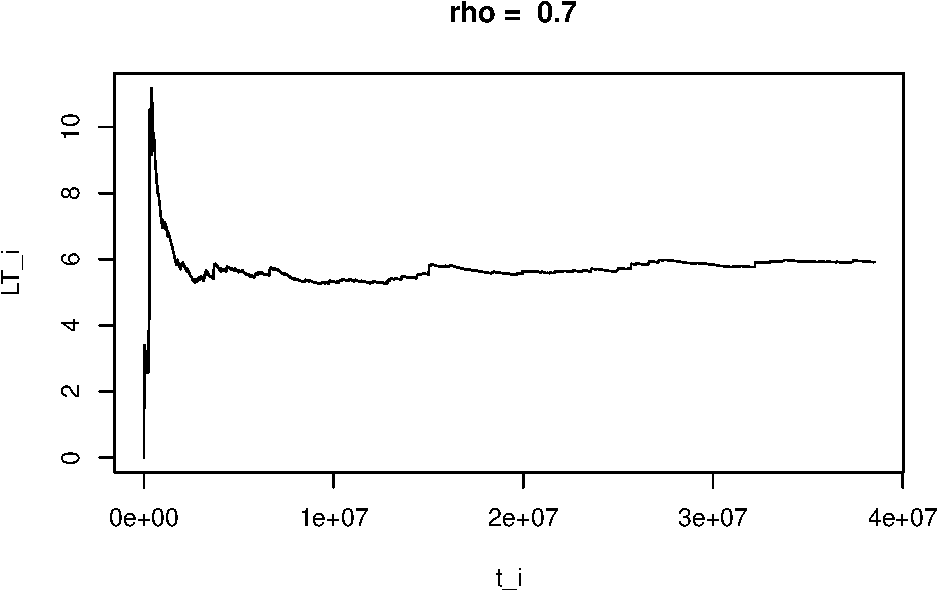
\includegraphics{003_files/figure-latex/unnamed-chunk-12-2.pdf}
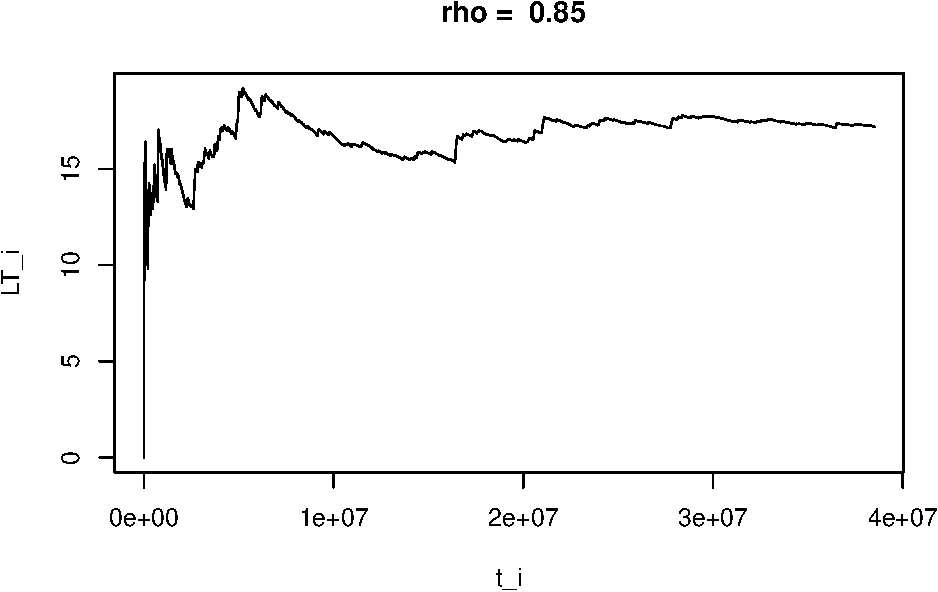
\includegraphics{003_files/figure-latex/unnamed-chunk-12-3.pdf}
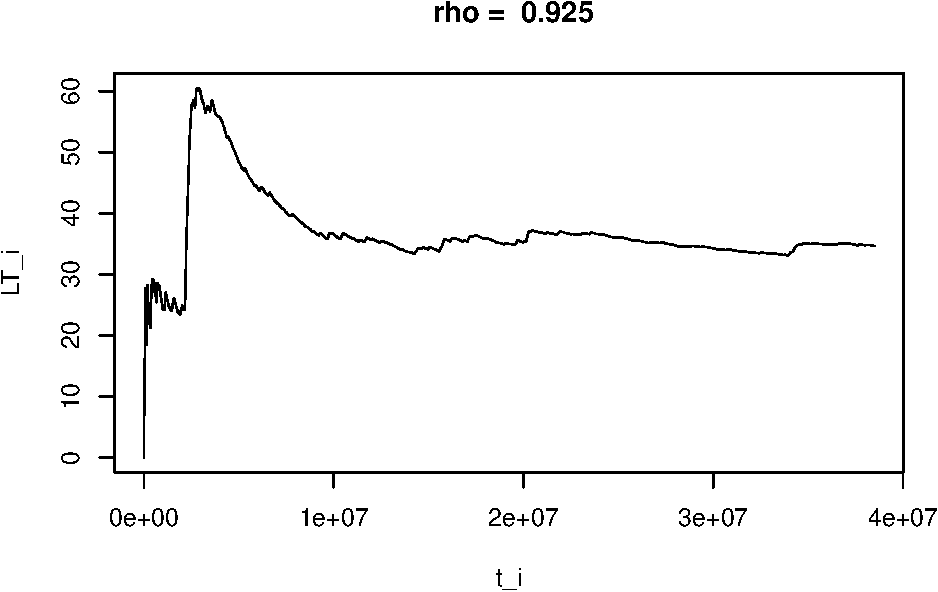
\includegraphics{003_files/figure-latex/unnamed-chunk-12-4.pdf}

\subsubsection{\texorpdfstring{\(\rho\) =
0.4}{\textbackslash{}rho = 0.4}}\label{rho-0.4}

We generate 10 simulations with 100000 clients, each with a different
seed. For each simulation, we check if the steady state is attained
without any abrupt increase or decrease in the value of the average
occupancy. In case there's any abrupt increase or decrease, we change
the seed. If for many seeds, this phenomena is still happening, we
increase the number of clients.

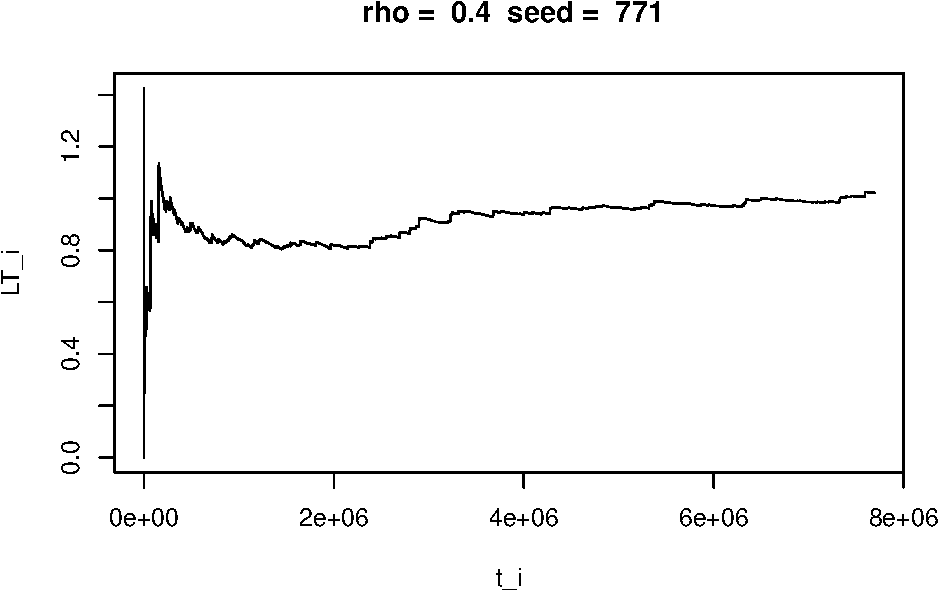
\includegraphics{003_files/figure-latex/unnamed-chunk-14-1.pdf}
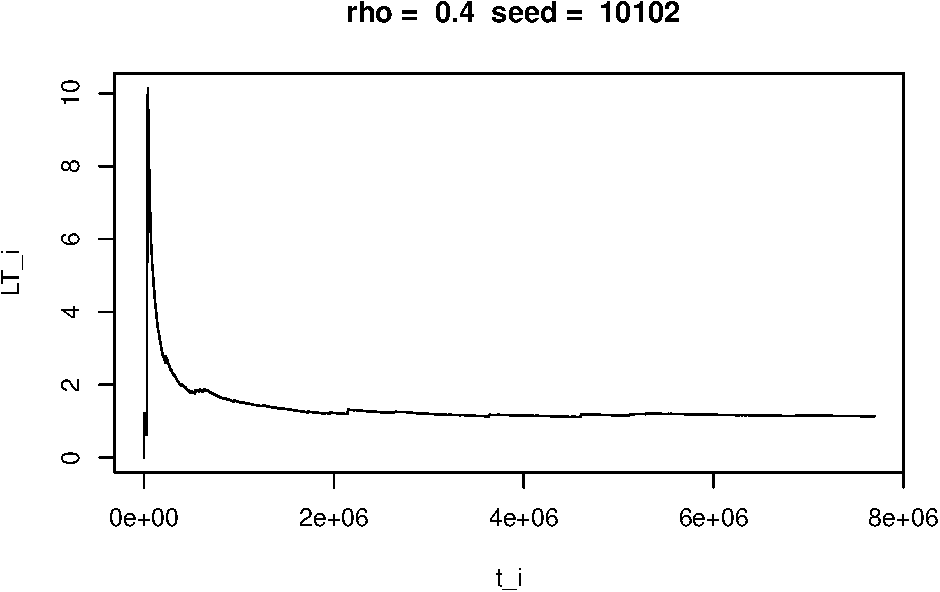
\includegraphics{003_files/figure-latex/unnamed-chunk-14-2.pdf}
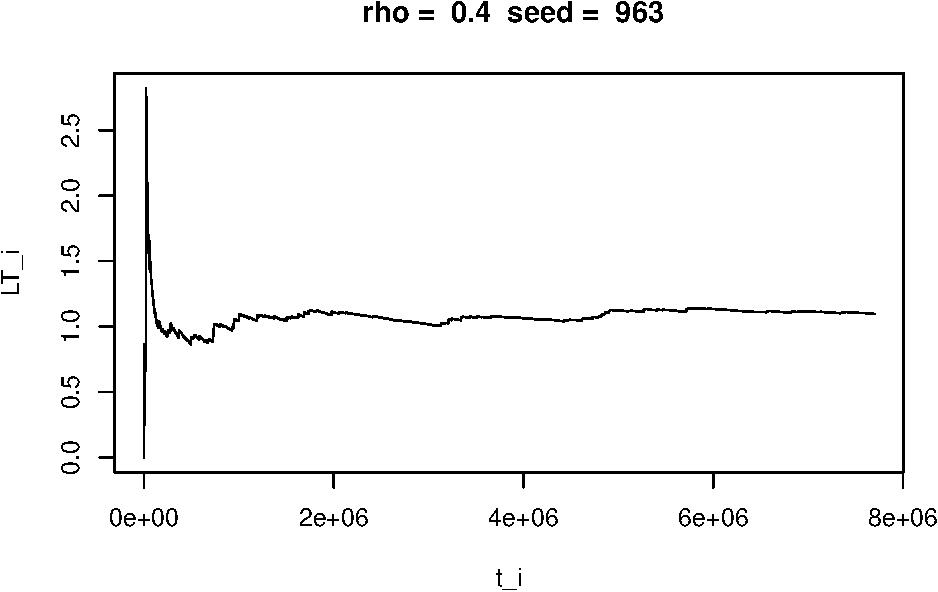
\includegraphics{003_files/figure-latex/unnamed-chunk-14-3.pdf}
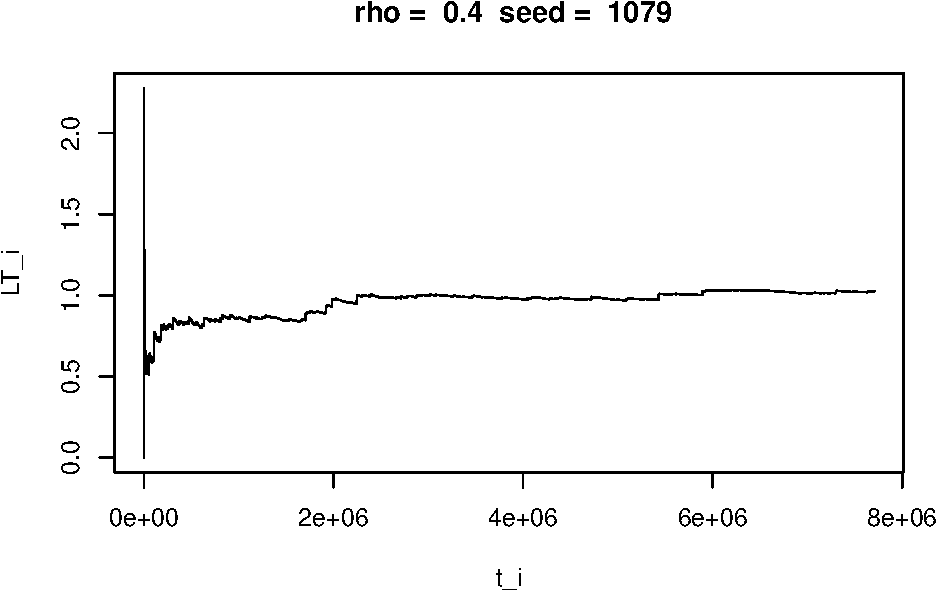
\includegraphics{003_files/figure-latex/unnamed-chunk-14-4.pdf}
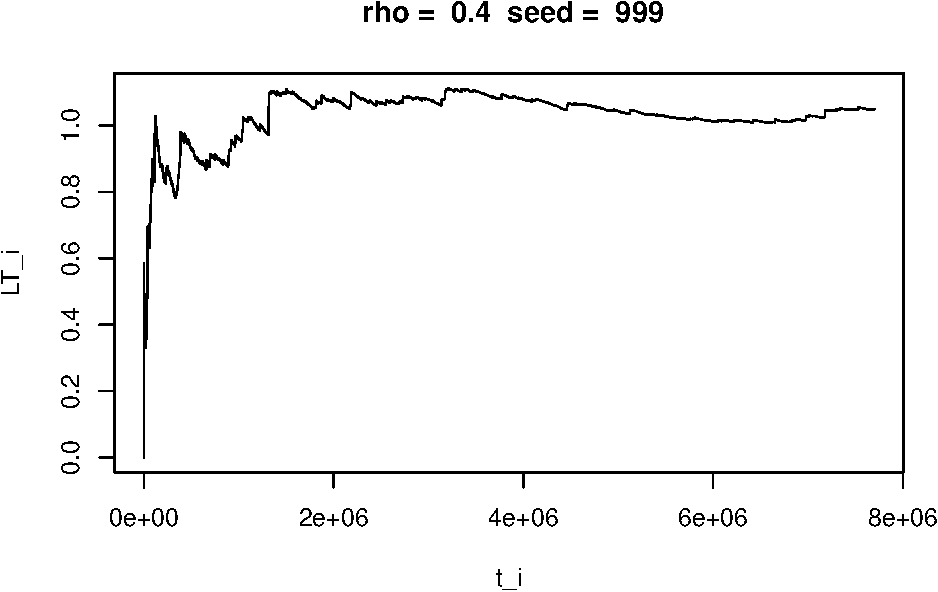
\includegraphics{003_files/figure-latex/unnamed-chunk-14-5.pdf}
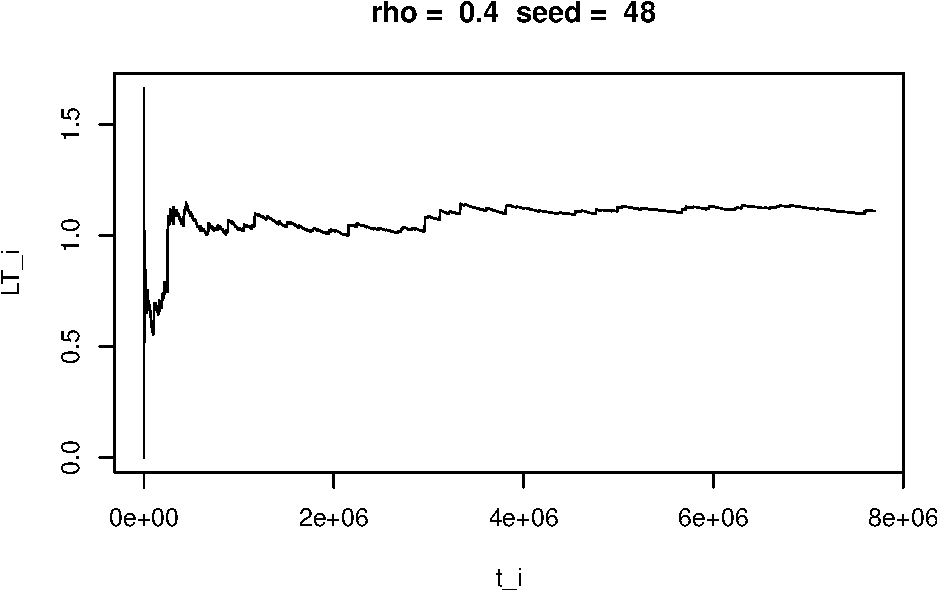
\includegraphics{003_files/figure-latex/unnamed-chunk-14-6.pdf}
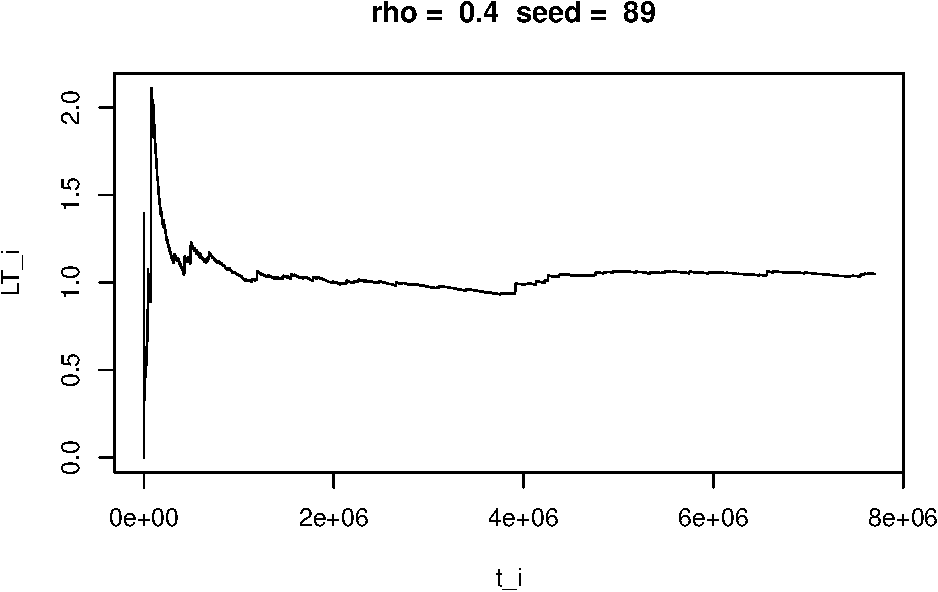
\includegraphics{003_files/figure-latex/unnamed-chunk-14-7.pdf}
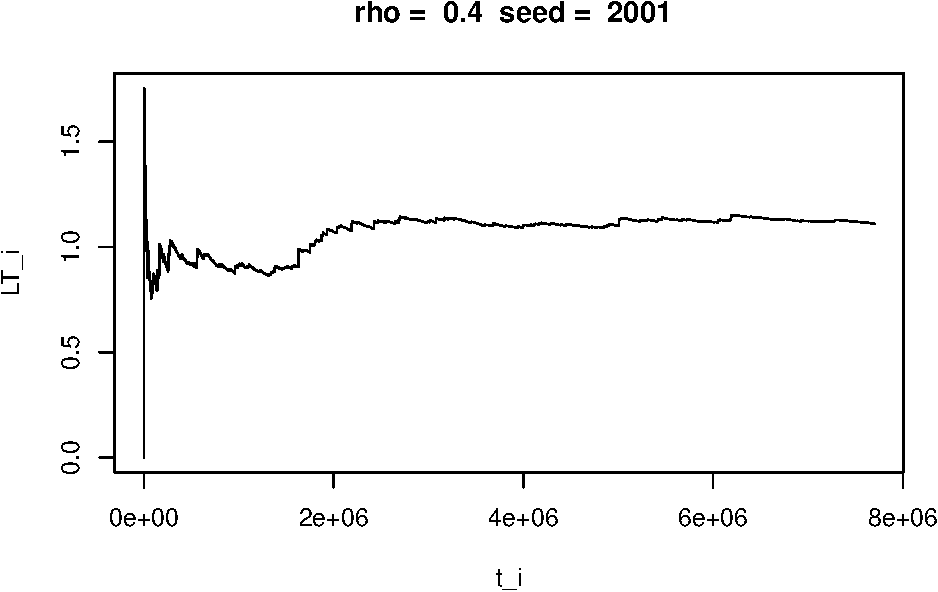
\includegraphics{003_files/figure-latex/unnamed-chunk-14-8.pdf}
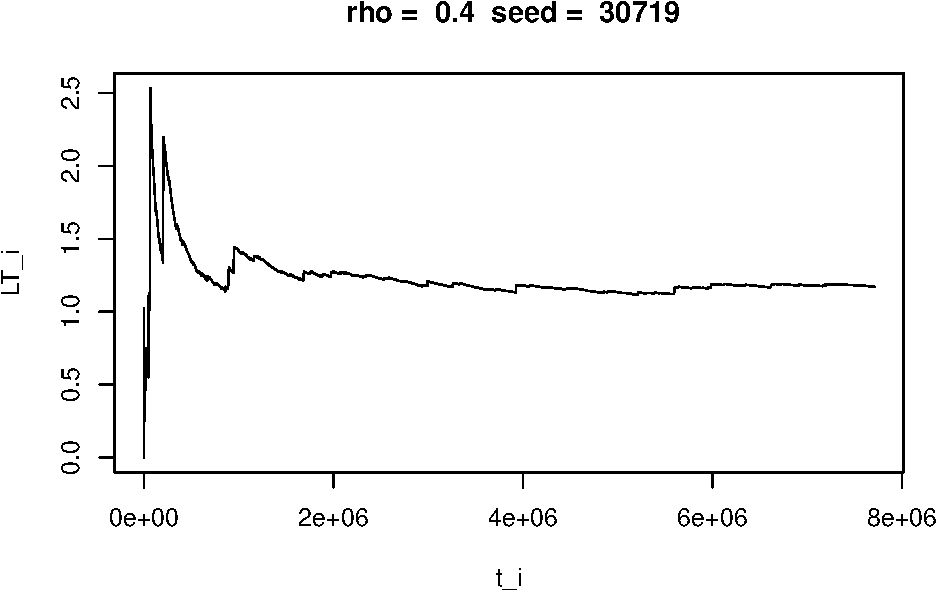
\includegraphics{003_files/figure-latex/unnamed-chunk-14-9.pdf}
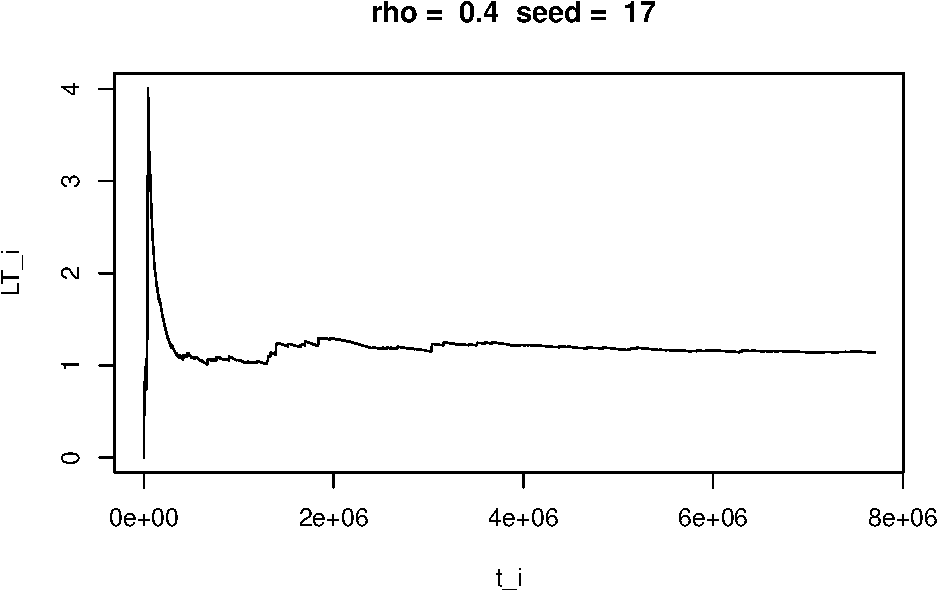
\includegraphics{003_files/figure-latex/unnamed-chunk-14-10.pdf}

We observe that for the seeds 10101, 1078, 960 and 51, there's an abrupt
change in the average occupancy. We change those seeds and redo the
simulation.

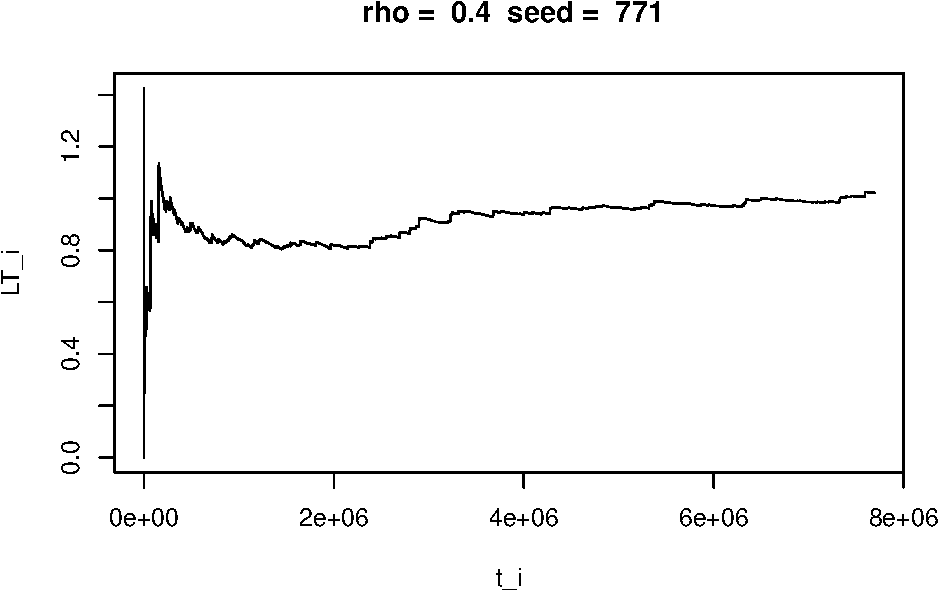
\includegraphics{003_files/figure-latex/unnamed-chunk-15-1.pdf}
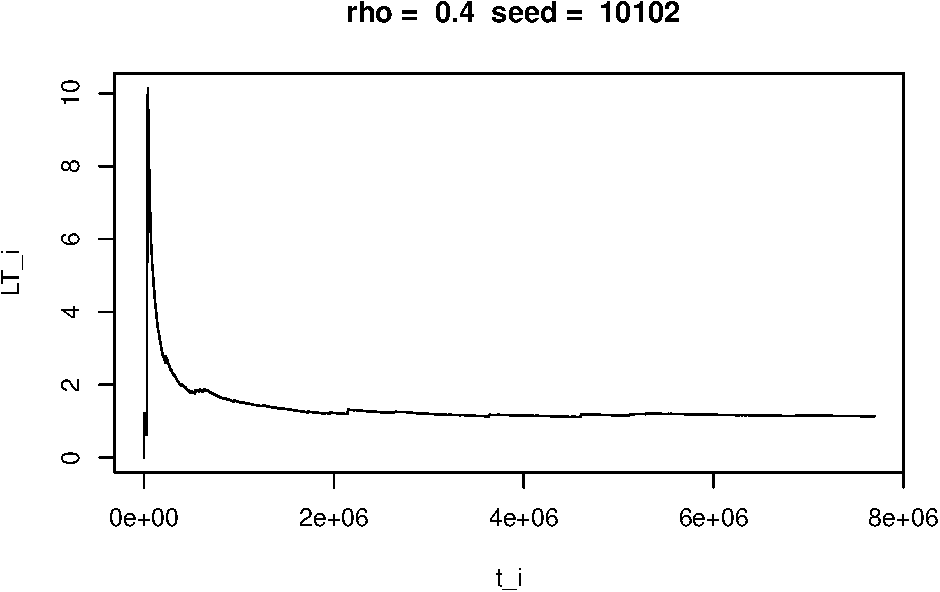
\includegraphics{003_files/figure-latex/unnamed-chunk-15-2.pdf}
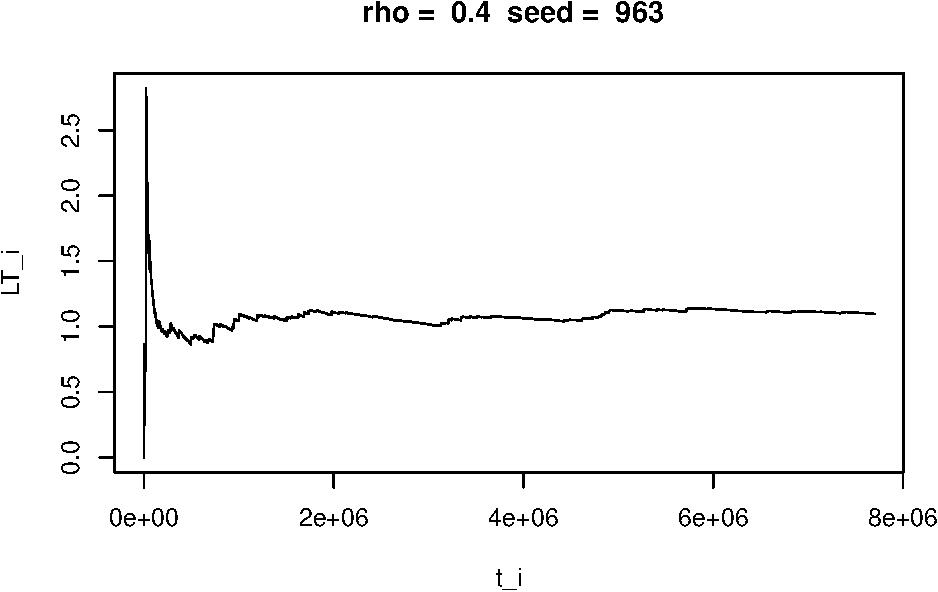
\includegraphics{003_files/figure-latex/unnamed-chunk-15-3.pdf}
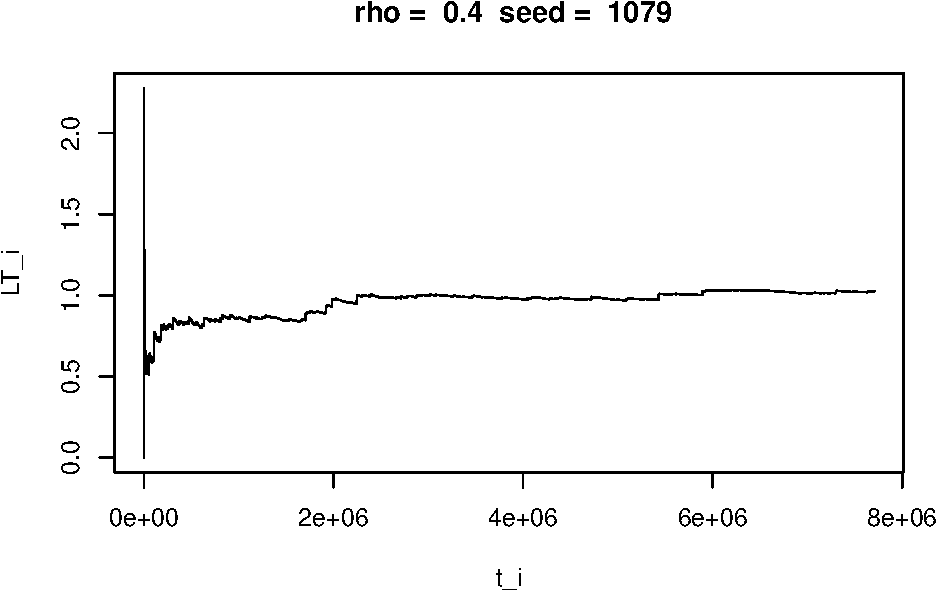
\includegraphics{003_files/figure-latex/unnamed-chunk-15-4.pdf}
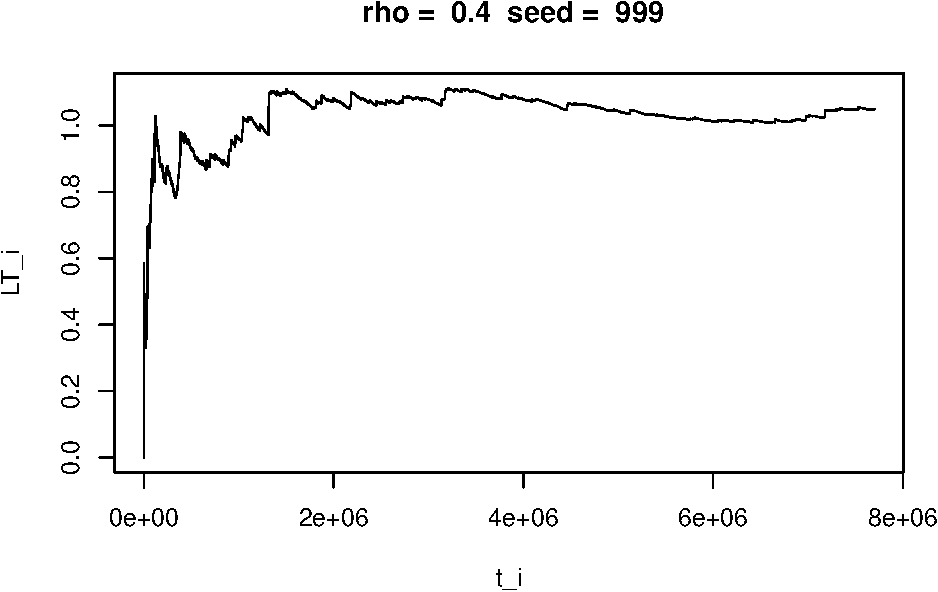
\includegraphics{003_files/figure-latex/unnamed-chunk-15-5.pdf}
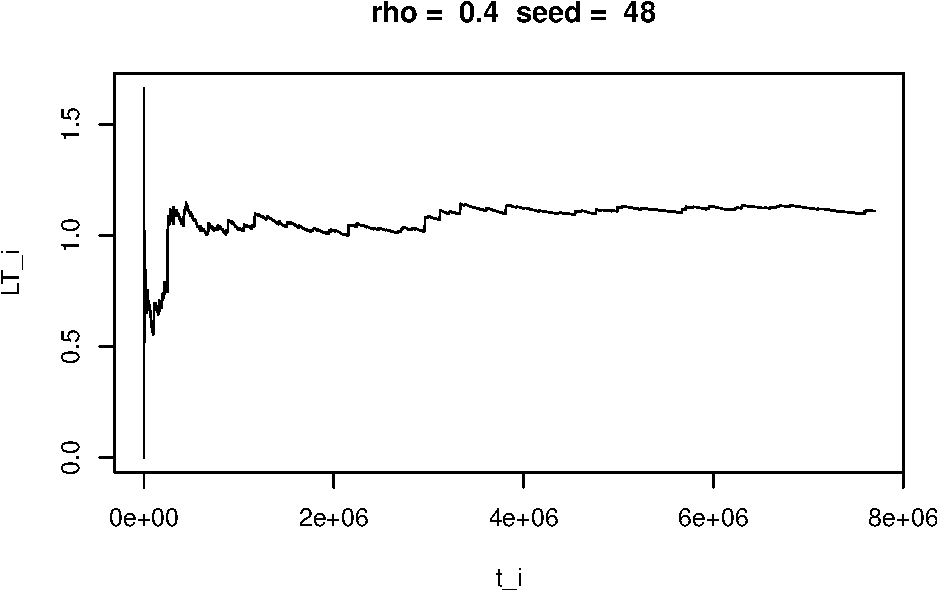
\includegraphics{003_files/figure-latex/unnamed-chunk-15-6.pdf}
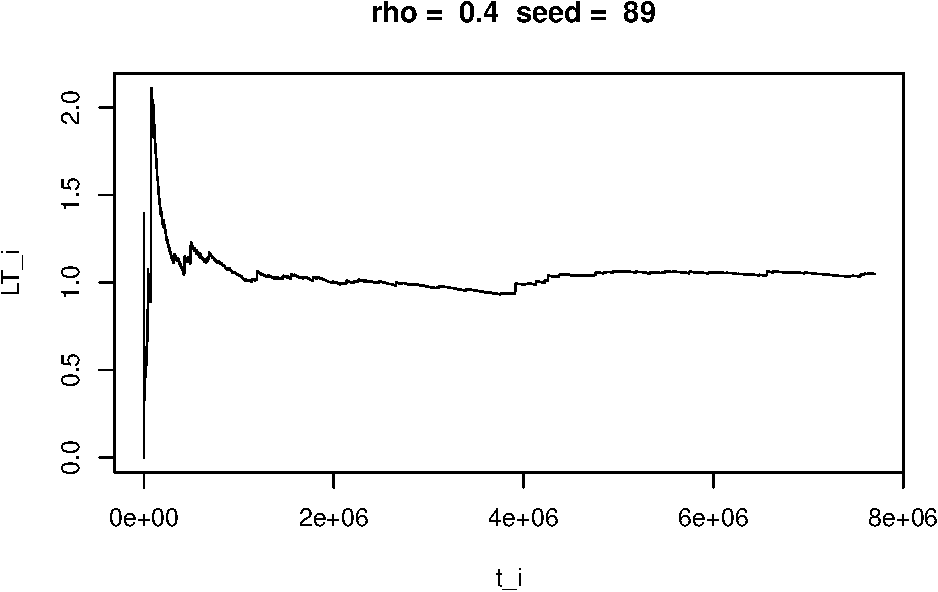
\includegraphics{003_files/figure-latex/unnamed-chunk-15-7.pdf}
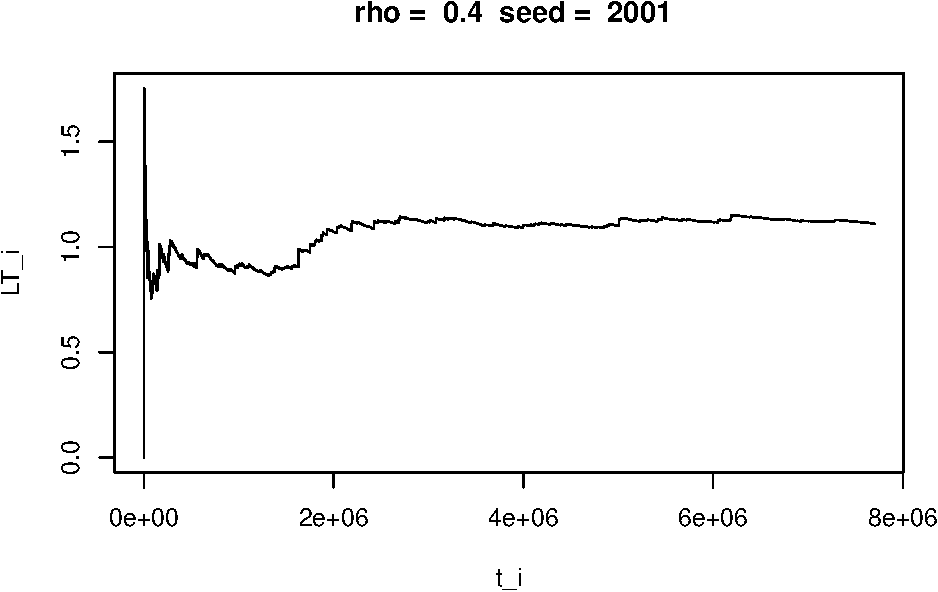
\includegraphics{003_files/figure-latex/unnamed-chunk-15-8.pdf}
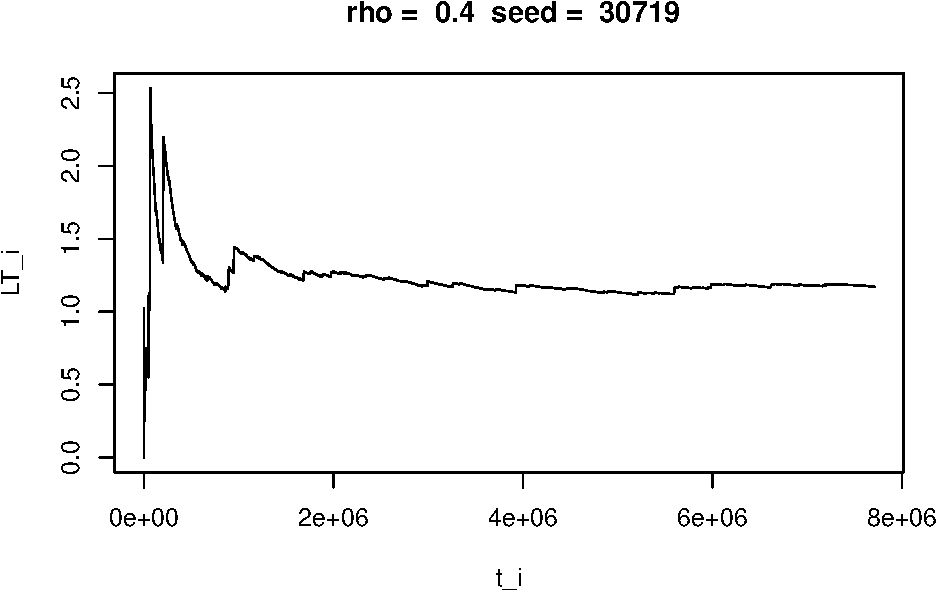
\includegraphics{003_files/figure-latex/unnamed-chunk-15-9.pdf}
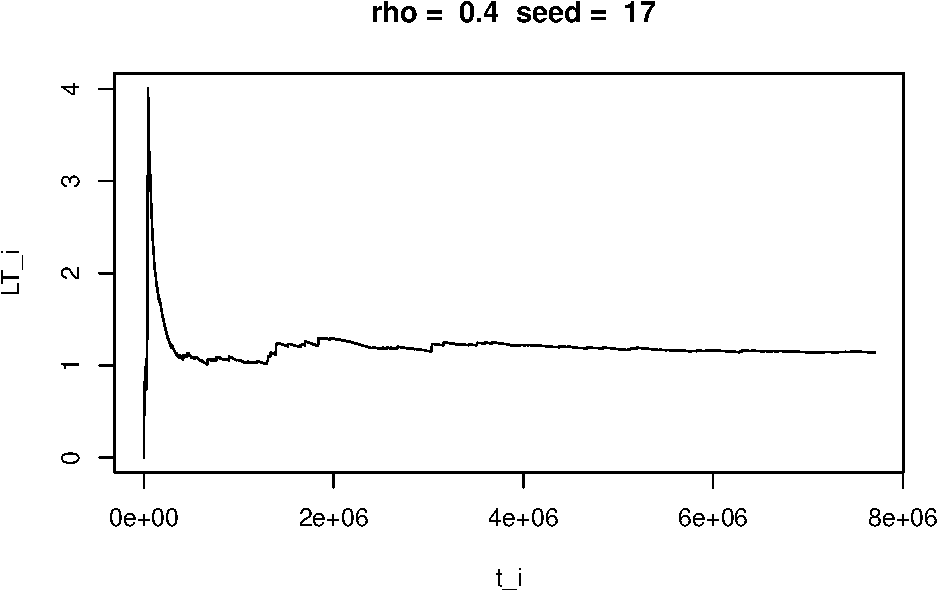
\includegraphics{003_files/figure-latex/unnamed-chunk-15-10.pdf}

We changed a total of 4 out of 10 seeds.

We now compute the confidence interval for \(L_{q}\) and \(W_{q}\). We
will use a t-Student distribution with critical value 1 - 0.95 and 9
degrees of freedom to compute a 95\% confidence interval.

\[
L_{q_{1}},L_{q_{2}},...,L_{q_{10}} \]
\[ \overline{L}_{q} = {1 \over n}\sum_{i=1}^{n}L_{q_{i}} \]
\[ S_{L_{q}}^{2} = {1 \over n - 1} \sum_{i=1}^{n} ( L_{q_{i}} - \overline{L}_{q} )^{2} \]
\[ C.I.(L_{q}) =   \overline{L}_{q} \pm t_{1 - \alpha, n - 1} \cdot \sqrt{S_{L_{q}}^{2} \over n} \]

\[
W_{q_{1}},W_{q_{2}},...,W_{q_{10}} \]
\[ \overline{W}_{q} = {1 \over n}\sum_{i=1}^{n}W_{q_{i}} \]
\[ S_{W_{q}}^{2} = {1 \over n - 1} \sum_{i=1}^{n} ( W_{q_{i}} - \overline{W}_{q} )^{2} \]
\[ C.I.(W_{q}) =   \overline{W}_{q} \pm t_{1 - \alpha, n - 1} \cdot \sqrt{S_{W_{q}}^{2} \over n} \]

The computations produce the followings confidence intervals for the
average queue length and waiting time:

\begin{verbatim}
##    NA        NA        NA       NA      NA
## 1 0.4 0.6629266 0.7216626 51.03537 55.5688
\end{verbatim}

\begin{longtable}[]{@{}llllll@{}}
\toprule
\(\rho\) & -C.I \(W_{q}\) & +C.I \(W_{q}\) & -C.I \(L_{q}\) & +C.I
\(L_{q}\) &\tabularnewline
\midrule
\endhead
0.4 & 0.6629266 & 0.7216626 & 51.0353731 & 55.5687961\tabularnewline
\bottomrule
\end{longtable}

\subsubsection{\texorpdfstring{\(\rho\) =
0.7}{\textbackslash{}rho = 0.7}}\label{rho-0.7}

We generate 10 simulations with 100000 clients, each with a different
seed. We check if the steady state is attained. We also check for
irregularities in the simulation results, in which case we change the
random number generator seed and repeat the simulation.

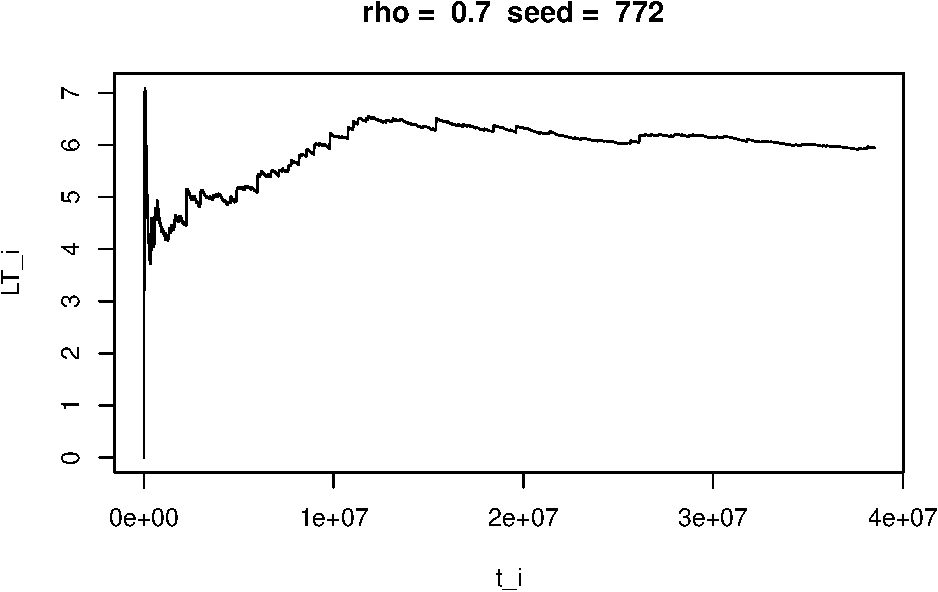
\includegraphics{003_files/figure-latex/unnamed-chunk-17-1.pdf}
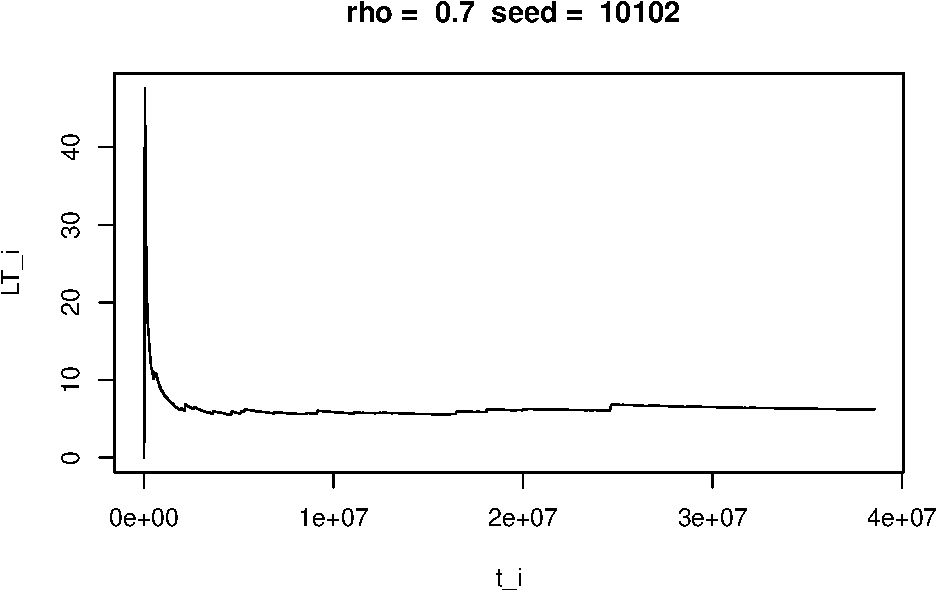
\includegraphics{003_files/figure-latex/unnamed-chunk-17-2.pdf}
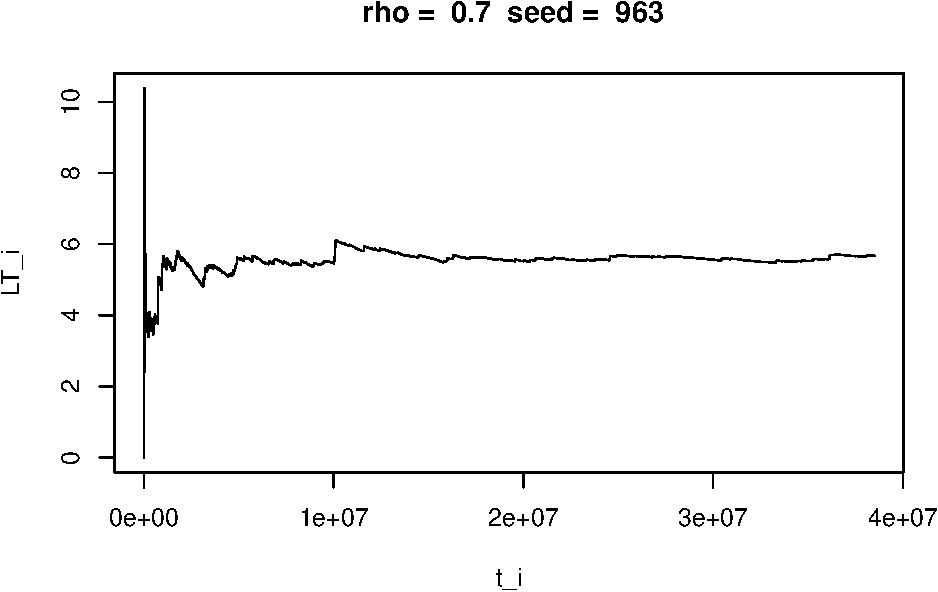
\includegraphics{003_files/figure-latex/unnamed-chunk-17-3.pdf}
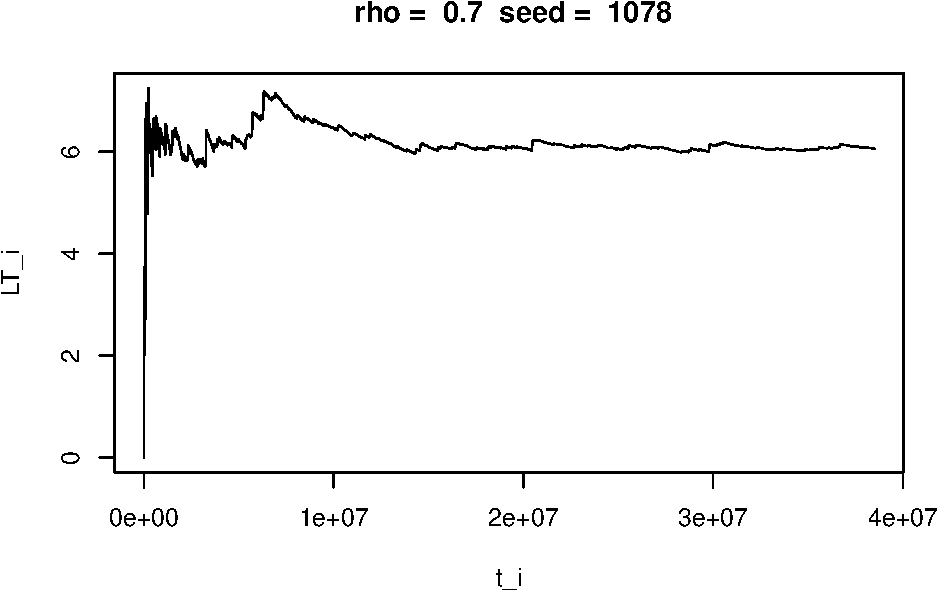
\includegraphics{003_files/figure-latex/unnamed-chunk-17-4.pdf}
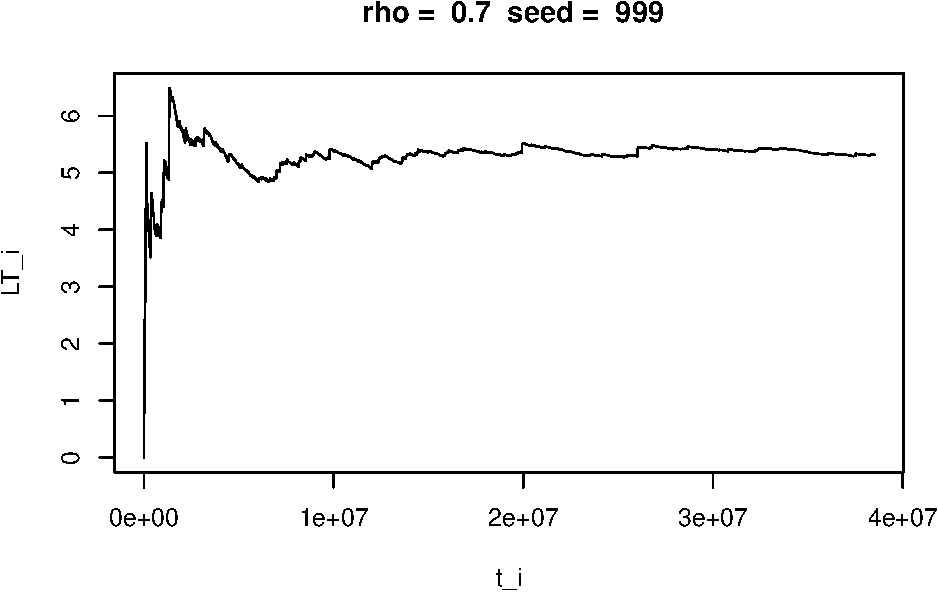
\includegraphics{003_files/figure-latex/unnamed-chunk-17-5.pdf}
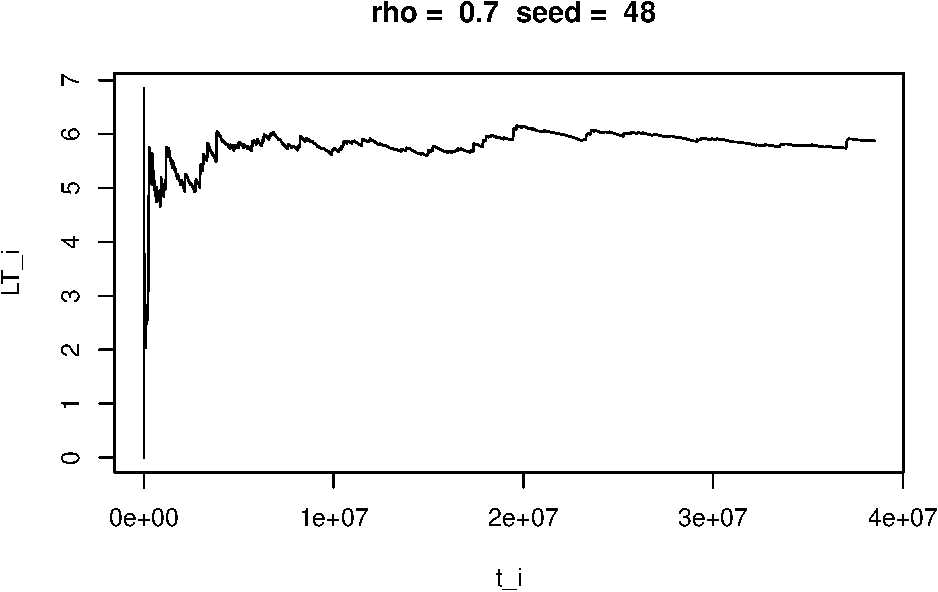
\includegraphics{003_files/figure-latex/unnamed-chunk-17-6.pdf}
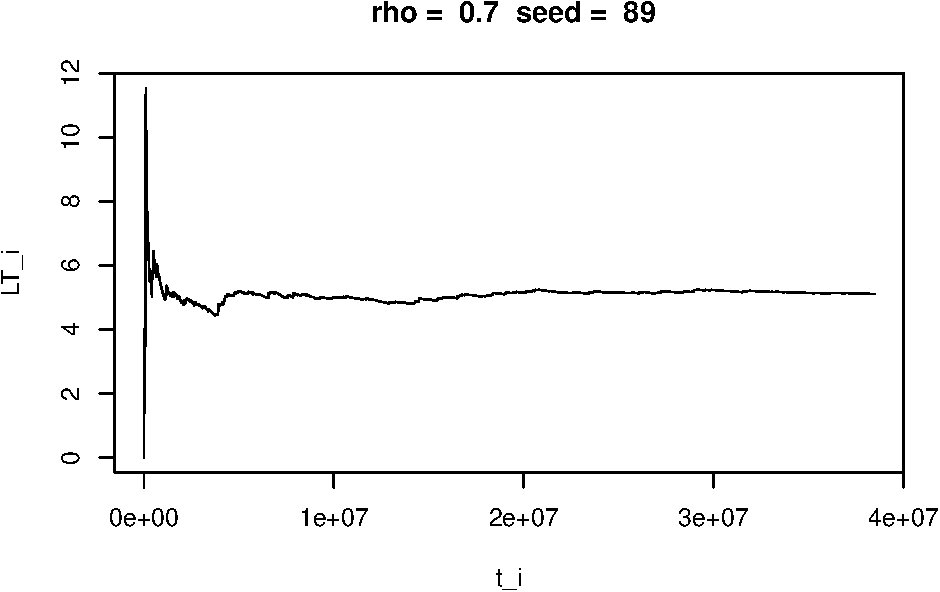
\includegraphics{003_files/figure-latex/unnamed-chunk-17-7.pdf}
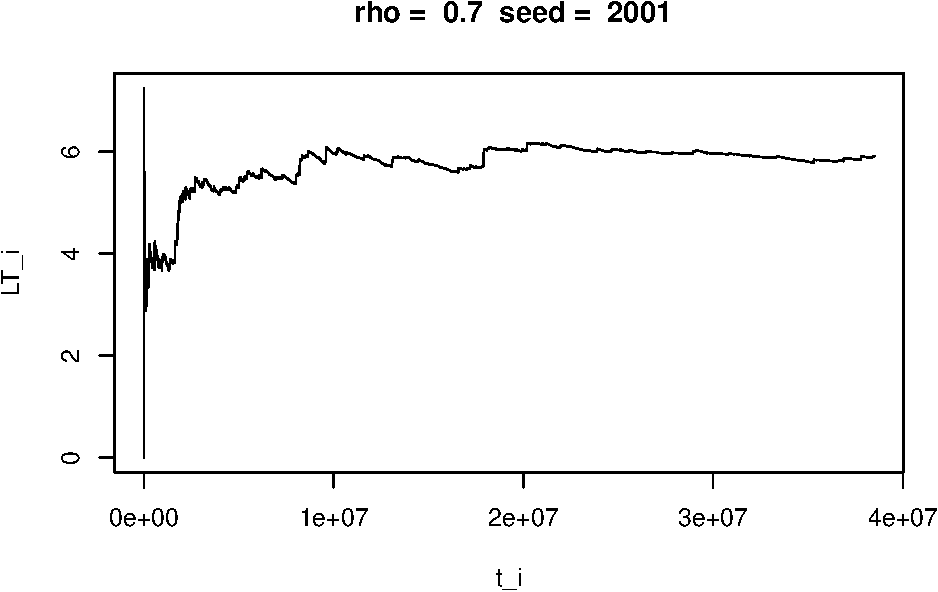
\includegraphics{003_files/figure-latex/unnamed-chunk-17-8.pdf}
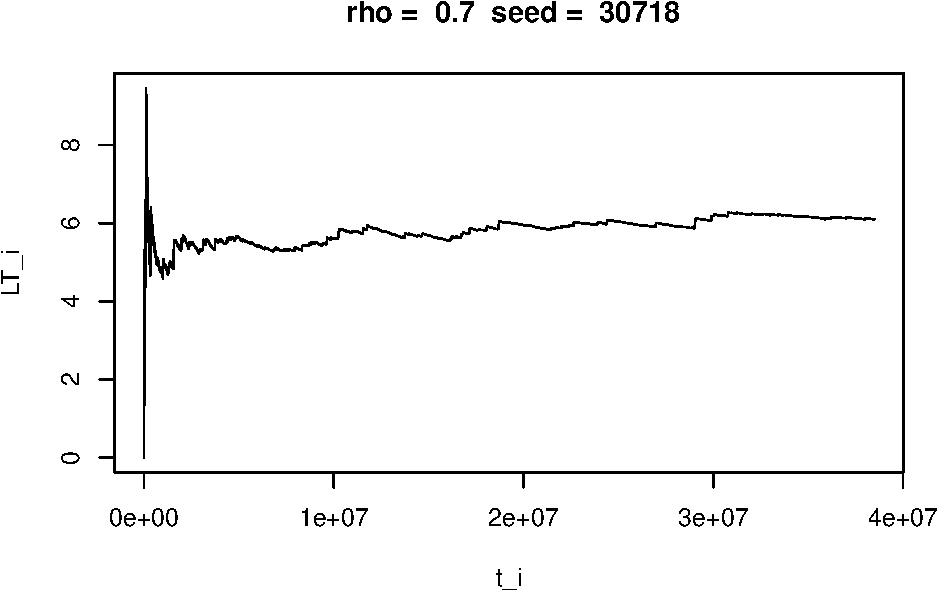
\includegraphics{003_files/figure-latex/unnamed-chunk-17-9.pdf}
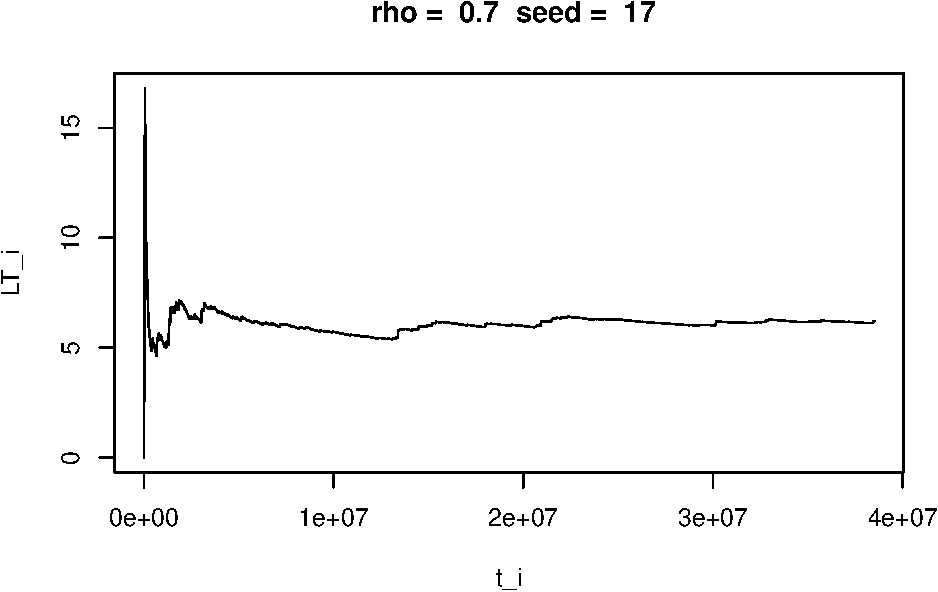
\includegraphics{003_files/figure-latex/unnamed-chunk-17-10.pdf}

We observe that 5 out of 10 simulations are not in a steady state at the
end of the simulation. We increase the number of clients to 500000 and
repeat the simulations.

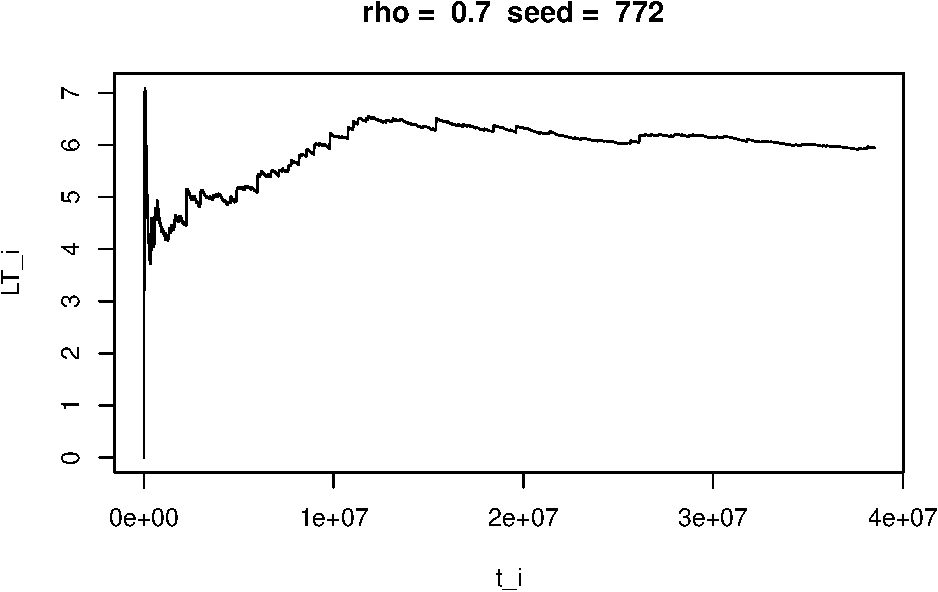
\includegraphics{003_files/figure-latex/unnamed-chunk-18-1.pdf}
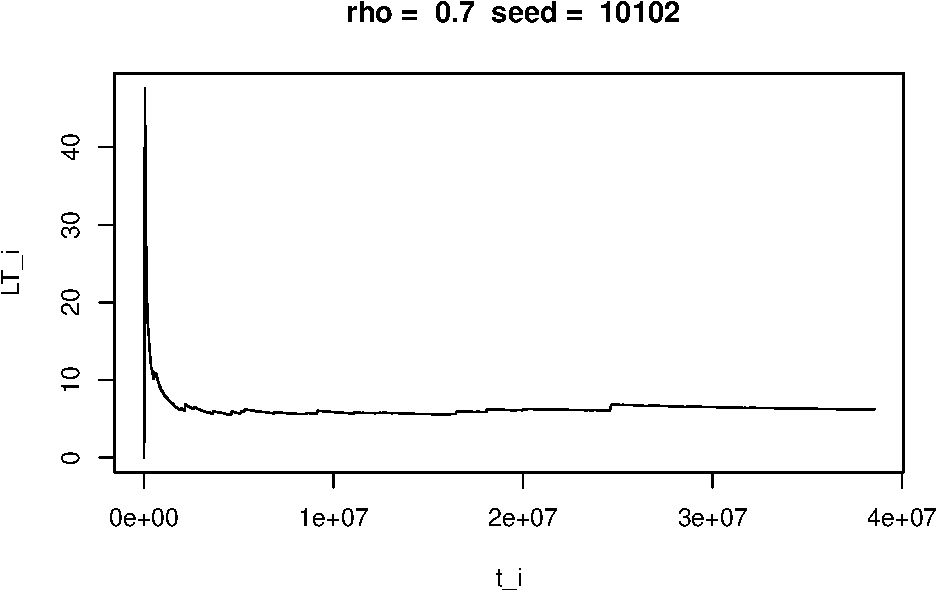
\includegraphics{003_files/figure-latex/unnamed-chunk-18-2.pdf}
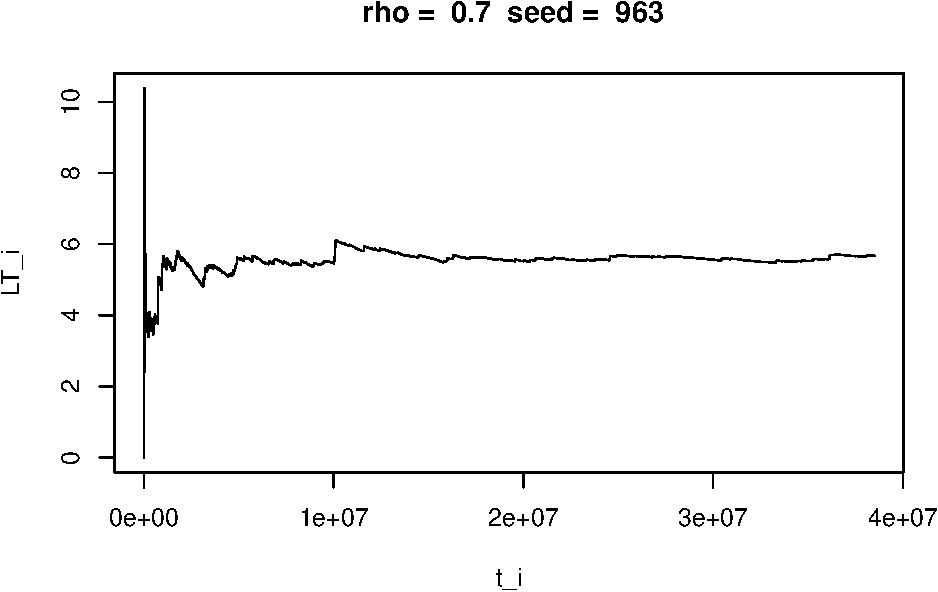
\includegraphics{003_files/figure-latex/unnamed-chunk-18-3.pdf}
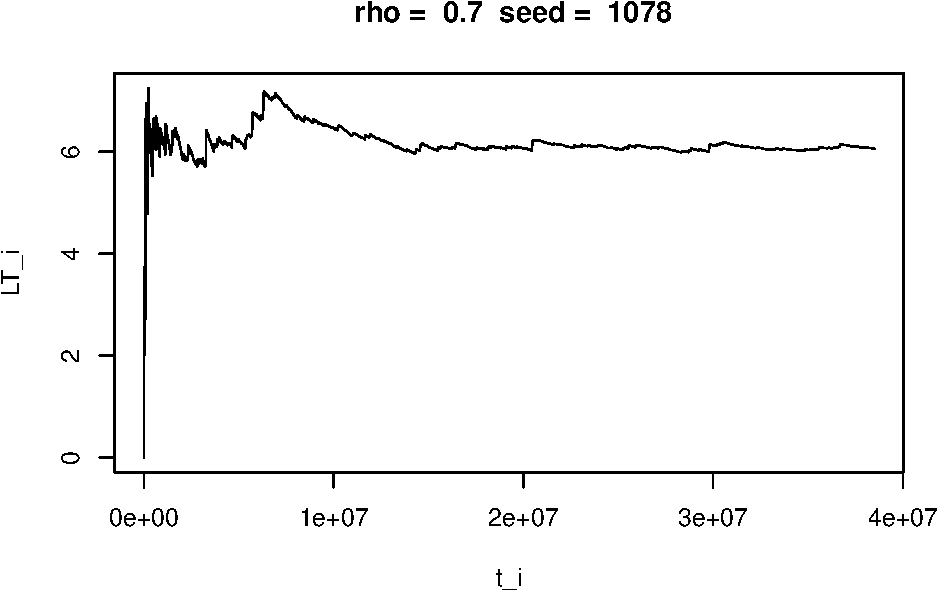
\includegraphics{003_files/figure-latex/unnamed-chunk-18-4.pdf}
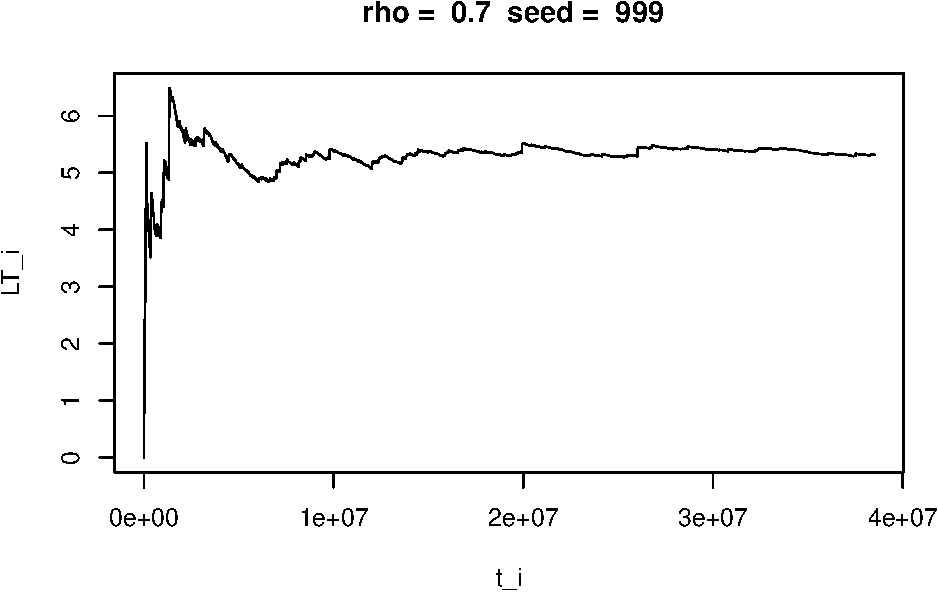
\includegraphics{003_files/figure-latex/unnamed-chunk-18-5.pdf}
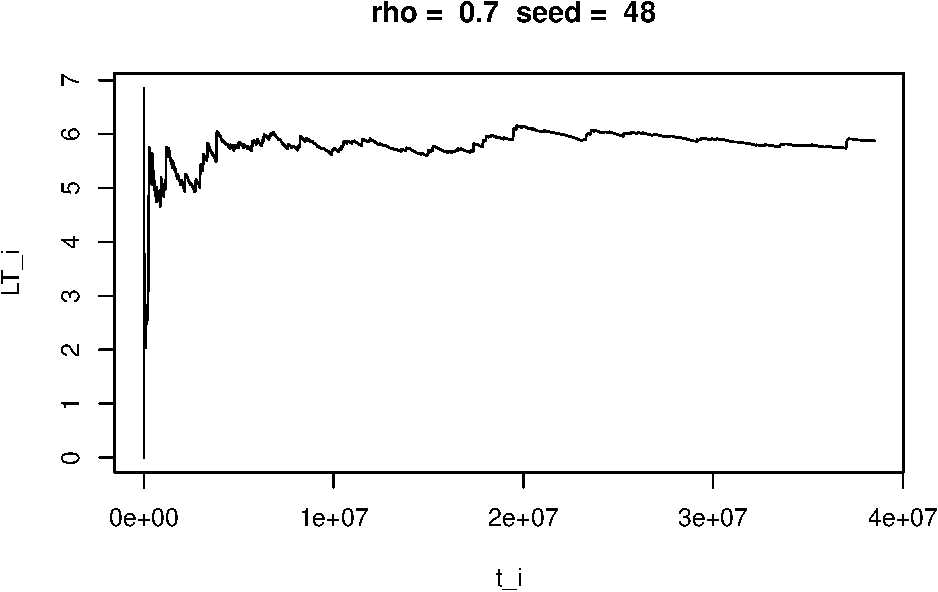
\includegraphics{003_files/figure-latex/unnamed-chunk-18-6.pdf}
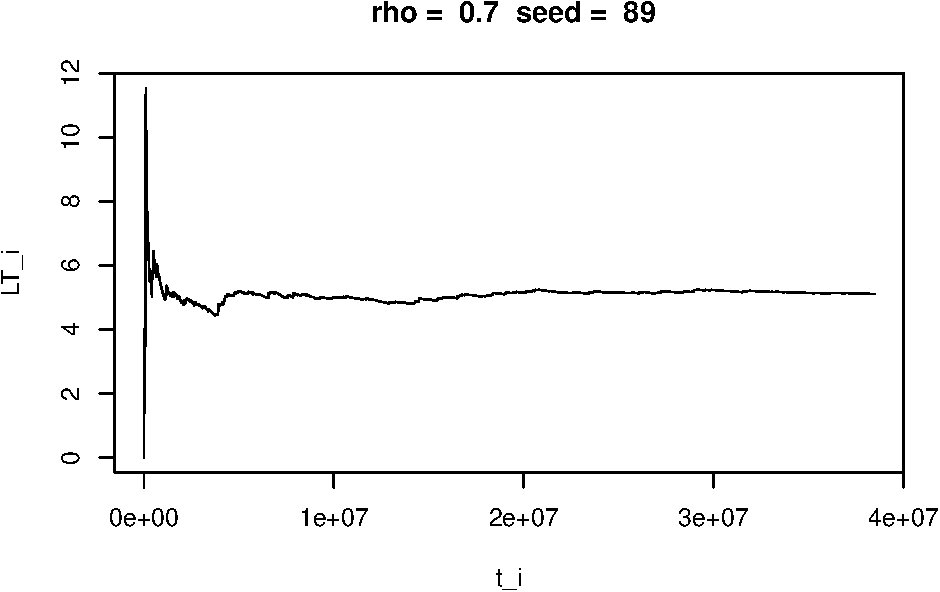
\includegraphics{003_files/figure-latex/unnamed-chunk-18-7.pdf}
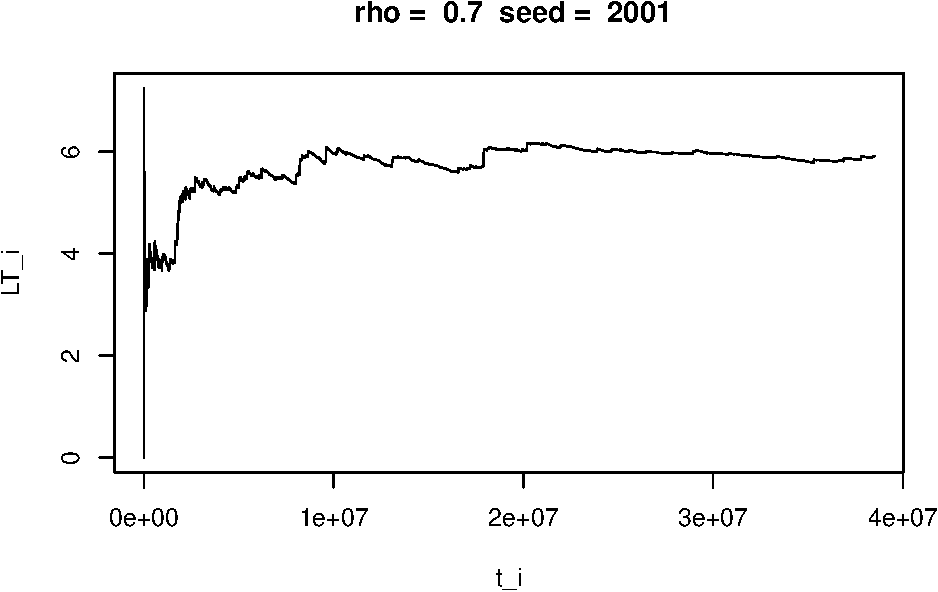
\includegraphics{003_files/figure-latex/unnamed-chunk-18-8.pdf}
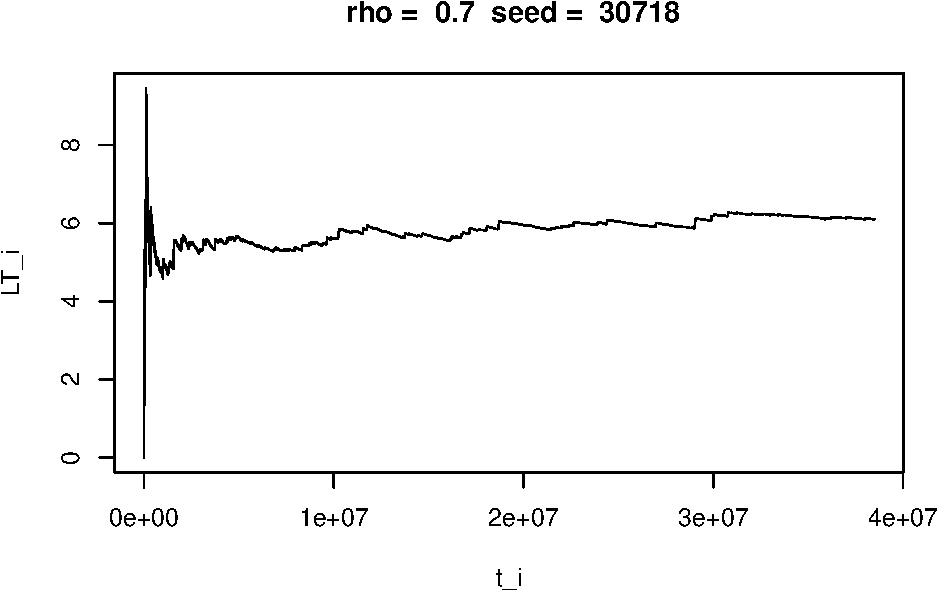
\includegraphics{003_files/figure-latex/unnamed-chunk-18-9.pdf}
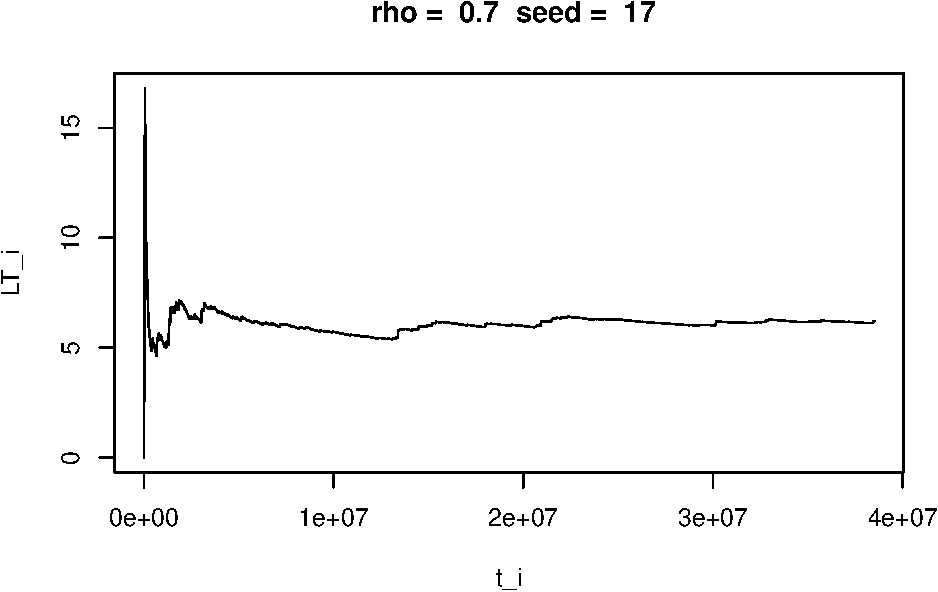
\includegraphics{003_files/figure-latex/unnamed-chunk-18-10.pdf}

We now compute the confidence interval for \(L_{q}\) and \(W_{q}\) using
the same procedure we detailed for \(\rho =\) 0.7. We will use a
t-Student distribution with critical value 1 - 0.95 and 9 degrees of
freedom to compute a 95\% confidence interval. The computations produce
the followings confidence intervals for the average queue length and
waiting time:

\begin{longtable}[]{@{}llllll@{}}
\toprule
\(\rho\) & -C.I \(W_{q}\) & +C.I \(W_{q}\) & -C.I \(L_{q}\) & +C.I
\(L_{q}\) &\tabularnewline
\midrule
\endhead
0.7 & 4.9266678 & 5.3560657 & 379.3389492 & 412.4915102\tabularnewline
\bottomrule
\end{longtable}

\subsubsection{\texorpdfstring{\(\rho\) =
0.85}{\textbackslash{}rho = 0.85}}\label{rho-0.85}

We generate 10 simulations with 100000 clients, each with a different
seed. We check if the steady state is attained. We also check for
irregularities in the simulation results, in which case we change the
random number generator seed and repeat the simulation.

\includegraphics{003_files/figure-latex/unnamed-chunk-20-1.pdf}
\includegraphics{003_files/figure-latex/unnamed-chunk-20-2.pdf}
\includegraphics{003_files/figure-latex/unnamed-chunk-20-3.pdf}
\includegraphics{003_files/figure-latex/unnamed-chunk-20-4.pdf}
\includegraphics{003_files/figure-latex/unnamed-chunk-20-5.pdf}
\includegraphics{003_files/figure-latex/unnamed-chunk-20-6.pdf}
\includegraphics{003_files/figure-latex/unnamed-chunk-20-7.pdf}
\includegraphics{003_files/figure-latex/unnamed-chunk-20-8.pdf}
\includegraphics{003_files/figure-latex/unnamed-chunk-20-9.pdf}
\includegraphics{003_files/figure-latex/unnamed-chunk-20-10.pdf}

We observe that seeds 963, 1078, 48 and 2001 produce irregularities in
the simulation, therefore we have to change them and repeat the
simulation.

\includegraphics{003_files/figure-latex/unnamed-chunk-21-1.pdf}
\includegraphics{003_files/figure-latex/unnamed-chunk-21-2.pdf}
\includegraphics{003_files/figure-latex/unnamed-chunk-21-3.pdf}
\includegraphics{003_files/figure-latex/unnamed-chunk-21-4.pdf}
\includegraphics{003_files/figure-latex/unnamed-chunk-21-5.pdf}
\includegraphics{003_files/figure-latex/unnamed-chunk-21-6.pdf}
\includegraphics{003_files/figure-latex/unnamed-chunk-21-7.pdf}
\includegraphics{003_files/figure-latex/unnamed-chunk-21-8.pdf}
\includegraphics{003_files/figure-latex/unnamed-chunk-21-9.pdf}
\includegraphics{003_files/figure-latex/unnamed-chunk-21-10.pdf}

We now compute the confidence interval for \(L_{q}\) and \(W_{q}\) using
the same procedure we detailed for \(\rho =\) 0.85. We will use a
t-Student distribution with critical value 1 - 0.95 and 9 degrees of
freedom to compute a 95\% confidence interval. The computations produce
the followings confidence intervals for the average queue length and
waiting time:

\begin{longtable}[]{@{}llllll@{}}
\toprule
\(\rho\) & -C.I \(W_{q}\) & +C.I \(W_{q}\) & -C.I \(L_{q}\) & +C.I
\(L_{q}\) &\tabularnewline
\midrule
\endhead
0.85 & 13.5934229 & 15.0731043 & 1046.5794927 &
1160.0665074\tabularnewline
\bottomrule
\end{longtable}

\subsubsection{\texorpdfstring{\(\rho\) =
0.925}{\textbackslash{}rho = 0.925}}\label{rho-0.925}

We generate 10 simulations with 100000 clients, each with a different
seed. We check if the steady state is attained. We also check for
irregularities in the simulation results, in which case we change the
random number generator seed and repeat the simulation.

\includegraphics{003_files/figure-latex/unnamed-chunk-23-1.pdf}
\includegraphics{003_files/figure-latex/unnamed-chunk-23-2.pdf}
\includegraphics{003_files/figure-latex/unnamed-chunk-23-3.pdf}
\includegraphics{003_files/figure-latex/unnamed-chunk-23-4.pdf}
\includegraphics{003_files/figure-latex/unnamed-chunk-23-5.pdf}
\includegraphics{003_files/figure-latex/unnamed-chunk-23-6.pdf}
\includegraphics{003_files/figure-latex/unnamed-chunk-23-7.pdf}
\includegraphics{003_files/figure-latex/unnamed-chunk-23-8.pdf}
\includegraphics{003_files/figure-latex/unnamed-chunk-23-9.pdf}
\includegraphics{003_files/figure-latex/unnamed-chunk-23-10.pdf}

We observe that \ldots{} PENDING \textless{}---- can we remove this?

We now compute the confidence interval for \(L_{q}\) and \(W_{q}\) using
the same procedure we detailed for \(\rho =\) 0.925. We will use a
t-Student distribution with critical value 1 - 0.95 and 9 degrees of
freedom to compute a 95\% confidence interval. The computations produce
the followings confidence intervals for the average queue length and
waiting time:

\begin{longtable}[]{@{}llllll@{}}
\toprule
\(\rho\) & -C.I \(W_{q}\) & +C.I \(W_{q}\) & -C.I \(L_{q}\) & +C.I
\(L_{q}\) &\tabularnewline
\midrule
\endhead
0.925 & 30.8481543 & 34.8003273 & 2375.1731581 &
2678.1414924\tabularnewline
\bottomrule
\end{longtable}

\subsection{Comparison of Allen Cuneen's approximation and the
simulation}\label{comparison-of-allen-cuneens-approximation-and-the-simulation}

\begin{longtable}[]{@{}llllllll@{}}
\toprule
\(\rho\) & \(W_{q}\) & -C.I \(W_{q}\) & +C.I \(W_{q}\) & \(L_{q}\) &
-C.I \(L_{q}\) & +C.I \(L_{q}\) &\tabularnewline
\midrule
\endhead
0.4 & 69.1507968 & 51.0353731 & 55.5687961 & 0.8980623 & 0.6629266 &
0.7216626\tabularnewline
0.7 & 423.5486306 & 379.3389492 & 412.4915102 & 5.5006316 & 4.9266678 &
5.3560657\tabularnewline
0.85 & 1249.0362678 & 1046.5794927 & 1160.0665074 & 16.2212502 &
13.5934229 & 15.0731043\tabularnewline
0.925 & 2958.3575269 & 2375.1731581 & 2678.1414924 & 38.4202276 &
30.8481543 & 34.8003273\tabularnewline
\bottomrule
\end{longtable}

As we can see in the table above Allen-Cuneen's approximation values for
all loading factors are outside of the confidence interval of our
simulations, always above. Overall, the approximations of both, \(W_q\)
and \(L_{q}\), are not very far from the simulation's confidence
interval.

So the Allen-Cuneen's aproximation models a system where the occupancy
is higher and the waiting times in the queue are also greater than what
our simulation produces. How can we explain that?

First of all, our random number generator has not been tested. As
discussed in class, it is impossible to generate real randomness, so
every rng must be tested for multiple desirable properties. In our
particular case, even though we used the rng that ships with R, which is
considered to ship with well tested generated random number streams, we
noticed that while repeatedly running the simulation we needed to change
the seed from time to time in order to avoid irregularities or abrupt
changes. We can conclude that we need to test the rng for appropriate
period, given that we need around 200.000 samples in each simulation.

Secondly, the Allen Cuneen's approximation uses the exact values for
exponential models and a correction factor for our model. Causes to the
difference between aproximation and simulation:

\begin{enumerate}
\def\labelenumi{\arabic{enumi}.}
\tightlist
\item
  Our model is not so close to a heavy tail distribution, so the
  correction factor is not accurate in the Allen Cuneen's formula.
\item
  We cannot use the Allen Cuneen's approximation formula with our model.
  We need to use the Kôllerstrôm formula, as our system is in ``heavy
  traffic'' conditions (it is a heavy tail distribution and that means
  heavy traffic?)
\item
  Something related to Ctau and Cx given that arrivals is a Normal
  distr. and service times is lognormal?
\end{enumerate}

\begin{longtable}[]{@{}llllllll@{}}
\toprule
\(\rho\) & \(W_{q}\) & -C.I \(W_{q}\) & +C.I \(W_{q}\) & \(L_{q}\) &
-C.I \(L_{q}\) & +C.I \(L_{q}\) &\tabularnewline
\midrule
\endhead
0.4 & 0.8336202 & 51.0353731 & 55.5687961 & 2.8977492 & 0.6629266 &
0.7216626\tabularnewline
0.7 & 1.6672404 & 379.3389492 & 412.4915102 & 17.6182641 & 4.9266678 &
5.3560657\tabularnewline
0.85 & 3.3344807 & 1046.5794927 & 1160.0665074 & 51.8958797 & 13.5934229
& 15.0731043\tabularnewline
0.925 & 6.6689615 & 2375.1731581 & 2678.1414924 & 122.8694038 &
30.8481543 & 34.8003273\tabularnewline
\bottomrule
\end{longtable}

We can observe that Köllerström formula does not apply to this
situation. We conclude that we are not in heavy traffic conditions.


\end{document}
